% !TeX root = main.tex
\documentclass[lettersize,journal]{IEEEtran}
\usepackage[caption=false,font=footnotesize]{subfig}
\usepackage{cite}
\usepackage{amsmath}
\usepackage{amssymb}
\usepackage{amsfonts}
\usepackage{graphicx}
\usepackage{algorithm,algorithmic}
\usepackage{hyperref}
\hypersetup{hidelinks=true}
\usepackage{textcomp}
\usepackage{booktabs}
\usepackage{multirow}
\usepackage{stfloats}
\usepackage{epstopdf}
\usepackage{titlesec}
\usepackage[table,xcdraw]{xcolor}

\setlength{\textfloatsep}{4pt plus 1.0pt minus 2.0pt}  
\setlength{\intextsep}{4pt plus 1.0pt minus 2.0pt}    
\setlength{\abovecaptionskip}{3pt}                    
\setlength{\belowcaptionskip}{0pt}
\setlength{\floatsep}{5pt}      
\setlength{\dblfloatsep}{5pt}   
\setlength{\parskip}{0pt}     
\setlength{\parindent}{1em}
\linespread{1.0}  
\titlespacing{\subsection}{0pt}{6pt}{5pt}
\markboth{IEEE Transactions on Multimedia, ~Vol.~14, No.~8, August~2025}%
{Wen \MakeLowercase{\textit{et al.}}: SMC-Net: Structure-Aware Multi-Scale Coarse-to-Fine Cascaded Network for Joint Choroid Layer and Vessel Segmentation}

\begin{document}

\title{SMC-Net: Structure-Aware Multi-Scale Coarse-to-Fine Cascaded Network for Joint Choroid Layer and Vessel Segmentation}

\author{Yang Wen, \IEEEmembership{Member, IEEE}, Shunzhe Shen, Lei Bi, Wuzhen Shi, \IEEEmembership{Senior Member, IEEE}, Ping Li, Bin Sheng, \IEEEmembership{Senior Member, IEEE}, and Xiaokang Yang, \IEEEmembership{Fellow, IEEE}

\thanks{This work was supported in part by the National Natural Science Foundation of China under Grant Nos. 62301330, in part by the Guangdong Basic and Applied Basic Research Foundation under Grant Nos. 2024A1515010496 and 2022A1515110101, in part by the Shenzhen Science and Technology Program under Grant Nos. 20231121103807001 and JCYJ20240813141358076, and in part by the Guangdong Provincial Key Laboratory under Grant Nos. 2023B1212060076.(Corresponding author: Wuzhen Shi).}
\thanks{Yang Wen, Shunzhe Shen and Wuzhen Shi are with Guangdong Provincial Key Laboratory of Intelligent Information Processing, College of Electronics and Information Engineering, Shenzhen University, Shenzhen, China (email: wen\_yang@szu.edu.cn; 2310433036@email.szu.edu.cn; wzhshi@szu.edu.cn.}
\thanks{Lei Bi is with the Translational medicine research institute, Shanghai Jiao Tong University, Shanghai, China (email: lei.bi@sjtu.edu.cn).}
\thanks{Ping Li is with the Department of Computing and the School of Design, The Hong Kong Polytechnic University, Hong Kong (email: p.li@polyu.edu.hk).}
\thanks{Bin Sheng is with the Department of Computer Science and Engineering, Shanghai Jiao Tong University, Shanghai, China (email: shengbin@sjtu.edu.cn).}
\thanks{Xiaokang Yang is with AI Institute, Shanghai Jiao
Tong University, Shanghai, China (email: xkyang@sjtu.edu.cn)}
}
         
\maketitle
\begin{abstract}  
Choroid thickness and choroidal vessel index are crucial biomarkers for the diagnosis, prediction, and treatment of various ophthalmic diseases.
{\color{red}However, high-noise OCT images hamper global structural modeling, leading to inconsistent vessel topology and morphology. Furthermore, existing cascaded frameworks often propagate errors by treating choroid layers and vessels in separate stages, neglecting their inherent anatomical relationships.}
{\color{red}To address these challenges, we propose SMC-Net, a structure-aware multi-scale coarse-to-fine cascaded network that employs Spatiocanal State Space Duality blocks to efficiently capture global spatial and channel-wise context for joint choroid layer and vessel segmentation.}
In the coarse stage, a Mamba-based U-shaped network is employed to segment the choroidal layer to provide a reliable prior for subsequent refinement.
In the refinement stage, a fractional-differential-based unsupervised prior extractor and Structure-Aware Modules are proposed to enhance subtle vascular structures in noisy OCT images.
Meanwhile, a structure-aware dual-branch network jointly models choroidal layer and vessel features to explicitly capture their anatomical relationships.
Finally, a choroidal edge-constrained joint loss is designed to enforce anatomical consistency between vessel and layer boundaries.
{\color{red}Extensive experiments on the private OCT-CCV dataset and the public RETOUCH dataset demonstrate the state-of-the-art performance and robust generalization of SMC-Net. Compared with the strongest choroid-specific baseline TACLNet under comparable computational cost, our SMC-Net-S improves fluid mIoU/DSC by 2.60\%/1.75\% on RETOUCH. Code will be available.}
\end{abstract}

\begin{IEEEkeywords}
Joint choroid layer and vessel segmentation, Structure-aware, State space duality, Coarse-to-fine cascaded network.
\end{IEEEkeywords}

\section{Introduction}
The choroid is essential for supplying oxygen and nutrients to the outer retina, and its thickness and vascular characteristics serve as important biomarkers for diagnosing, predicting, and monitoring ophthalmic conditions, such as age‑related macular degeneration and choroidal neovascularization~\cite{Singh2019Choroidal}.
Quantitative analysis of choroidal vessel enables clinicians to assess pathological changes and treatment efficacy more objectively.
However, accurate choroidal vessel segmentation remains challenging due to inherent characteristics of optical coherence tomography (OCT) images, including severe noise, imaging artifacts, and low contrast~\cite{tmm_3,tmm_7}.

Although previous methods~\cite{choroidnet,wen2024} in choroidal segmentation are impressive, the following issues remain unresolved. First, conventional choroidal cascaded segmentation paradigms are susceptible to error propagation, as inaccuracies in the initial choroid‑layer segmentation directly degrade subsequent vessel segmentation.
Additionally, such pipelines treat choroid layer and vessel segmentation as independent stages, failing to capture their inherent anatomical interdependence. Second, most approaches insufficiently incorporate structural priors of choroidal vessels, leading to compromised topological consistency and morphological fidelity in the segmentation results, despite evidence that structural information significantly improves performance in medical segmentation tasks~\cite{BEFD,structure_driven,dual_encoder_edge}.
Third, current CNN‑based choroidal segmentation methods are constrained by their limited global receptive fields ~\cite{Liu2019refine,choroidnet}. While Wen \textit{et al.}~\cite{wen2024} utilized a Transformer~\cite{vit} branch to provide sufficient global dependency modeling capacity, it led to a significant increase in the computational burden.
Consequently, these models for choroidal vessel segmentation always lack an efficient mechanism to model long‑range dependencies while maintaining practical usability.

To address these limitations, we propose SMC-Net, a structure-aware joint segmentation framework for choroidal vessel segmentation. Rather than treating choroidal layer and vessel segmentation as independent stages, SMC-Net explicitly models their anatomical dependency within a coarse-to-fine paradigm to mitigate error propagation. In the coarse stage, a Mamba-based U-shaped network~\cite{gu2024mamba} provides a reliable choroidal structural prior that suppresses noise and non-choroidal artifacts. In the refinement stage, a structure-aware dual-branch network jointly segments the choroidal layer and vessels, leveraging their anatomical correlation to enhance segmentation accuracy and boundary plausibility.

To further improve topological consistency under severe OCT noise, we introduce a fractional differential–based unsupervised edge detector to extract robust choroidal structural cues. Unlike conventional integer-order operators, the proposed detector enhances subtle vessel boundaries while avoiding excessive noise amplification. These structural cues are injected into semantic feature representations through dedicated Structure-Aware Modules (SAMs), enabling anatomically consistent vessel refinement. Moreover, to efficiently capture long-range dependencies, we incorporate a Spatiocanal State Space Duality (SSSD) mechanism~\cite{dao2024transformers} with linear complexity, which jointly models spatial and inter-channel dependencies by extending State Space Duality from natural language processing to choroidal OCT segmentation. Finally, a choroidal edge-constrained joint loss is designed to explicitly enforce consistency between vessel boundaries and choroidal layer boundaries.

The main contributions can be summarized as follows:
\begin{itemize}
    \item We propose a coarse-to-fine cascaded network (SMC-Net) for joint choroidal layer and vessels segmentation. SMC-Net uses an SSD-based U-shape network for coarse segmentation to filter artifacts and noise, and a structure-aware dual-branch network for refining segmentation. We also propose a choroidal edge-constrained joint loss function to further enhance performance by aligning vessel boundaries with choroidal layer boundaries.
    \item We design a novel fractional-differential-based unsupervised prior edge detector to accurately extract the structure information of choroidal vessels in high-noise OCT images. We also propose the Structure-Aware Modules (SAMs) to inject the detected vascular structure information into the OCT image features, ultimately improving the segmentation performance of complex vascular edges.
    \item We propose the SSSD blocks to achieve efficient long-range modeling, adapting SSD to model both spatial information and channel-wise information of choroidal features. To the best of our knowledge, our proposed SMC-Net method is the first to apply State Space Duality to the field of choroidal segmentation.
    \item We conduct extensive quantitative and qualitative experiments on a private choroidal vessel dataset and a public retinal segmentation benchmark, demonstrating the effectiveness and superiority of SMC-Net over state-of-the-art methods.
\end{itemize}

\section{Related Works}

\subsection{Deep-Learning Methods for Choroid Segmentation}
Traditional methods for choroidal layer and vessel segmentation exhibit limited robustness and are highly sensitive to pathological variations, leading to unsatisfactory performance~\cite{tmm_satnet_1,tmm_4,tmm_5}.
With advances in deep learning for medical image segmentation~\cite{tmm_8}, several dedicated models for choroidal analysis have been proposed.
Liu \textit{et al.}~\cite{Liu2019refine} introduced a deep learning-based approach for choroidal vessel segmentation, while Khaing \textit{et al.}~\cite{choroidnet} proposed ChoroidNET, a cascaded U-Net framework that first segments the choroidal layer and subsequently refines vessel segmentation.
More recently, Wen \textit{et al.}~\cite{wen2024} employed a two-stage architecture with a Shunted Transformer-enhanced U-Net and multi-scale fusion for vessel segmentation.
Despite their effectiveness, these approaches suffer from three key limitations: increased computational cost due to multi-stage designs, limited global context modeling, and inefficient resource utilization relative to performance gains.
These drawbacks motivate the development of a more efficient and robust segmentation framework.

\subsection{SSM-Based Methods for Medical Image Segmentation}
CNN-based methods are limited by their local receptive fields, which hampers long-range dependency modeling~\cite{tmm_2,tmm_6}, while Transformer-based approaches achieve global context modeling at the cost of quadratic computational complexity.
Recently, State Space Models (SSMs) have gained attention for their efficiency in modeling long sequences. Mamba~\cite{gu2024mamba} enhances structured SSMs through a selective mechanism and hardware-aware optimization, while its successor Mamba2~\cite{dao2024transformers} introduces SSD, unifying SSMs and structured masked attention via matrix multiplication for accelerated training. Subsequent studies have explored SSD-based architectures in vision tasks~\cite{shi2024vssdvisionmambanoncausal}, demonstrating their effectiveness.
However, existing SSD-based models remain suboptimal for choroidal segmentation, as OCT images are severely affected by noise and artifacts, posing challenges beyond those encountered in general medical imaging.

\subsection{Structure-Aware Methods in Medical Imaging}
In medical image segmentation, accurate delineation of region-of-interest (ROI) boundaries is crucial for structural analysis, motivating extensive efforts to enhance anatomical boundary perception.
Zhang \textit{et al}.~\cite{BEFD} employed Sobel-based boundary enhancement, while Cui \textit{et al}.~\cite{structure_driven} integrated Canny-detected boundaries with high-level structural features to guide cardiac segmentation.
Similarly, Li \textit{et al}.~\cite{dual_encoder_edge} designed a multi-directional Sobel-based edge encoder to extract structural cues.
These studies demonstrate that incorporating unsupervised edge information into deep learning frameworks can effectively strengthen structural representation in segmentation tasks.
However, choroidal OCT images suffer from severe noise and weak vessel boundaries, rendering conventional integer-order edge operators highly noise-sensitive and ineffective in capturing fine vascular details.


\section{Methodology}
The SMC-Net we proposed is shown in Fig.~\ref{fig:overview}.
It mainly includes the pretrained coarse segmentation stage and the refinement segmentation stage.

\begin{figure*}[!ht]
    \centering
    \includegraphics[width=0.96\textwidth]{fig/overview.pdf}
    \caption{Overview of the proposed \textbf{SMC-Net}.
    (a) Structural Information Encoder,
    (b) OCT Image Encoder,
    (c) Structure-Aware Phase,
    (d) Multi-Scale Commingling Attention Module (MCAM),
    and (e) Choroid Joint Decoder.
    SMC-Net consists of a pretrained coarse segmentation stage and a refinement stage.
    The coarse stage employs an SSD-based U-Net to generate initial choroidal layer masks, which are combined with OCT images and UPED priors for refinement.
    In the refinement stage, masked inputs are processed by Structure-Aware Modules to enhance vascular structures and by MCAM to integrate multi-scale features.
    Finally, a joint decoder produces choroidal layer and vessel segmentations, supervised by a joint loss enforcing anatomical boundary consistency.
    }

    \label{fig:overview}
\end{figure*}

\subsection{Pretrained Coarse Segmentation Stage}
{\color{red}For an input OCT image $x \in \mathbb{R}^{H \times W \times 3}$, the structural information $s$ is extracted by the proposed unsupervised prior edge detector $\text{UPED}$: $s = \text{UPED}(x)$, $s \in \mathbb{R}^{H \times W \times 3}$. The pretrained coarse segmentation network $\varPhi_{\text{Pre}}(\cdot)$ produces a coarse choroidal mask $m_c = \varPhi_{\text{Pre}}(x)$, which is applied to both the original OCT image $x$ and the extracted structural information $s$ to obtain region-of-interest inputs for the refinement stage:
$x_{\text{masked}} = m_c \cap x, \quad s_{\text{masked}} = m_c \cap s,$ where $x_{\text{masked}}, s_{\text{masked}} \in \mathbb{R}^{H \times W \times 1}$.
By restricting the refinement stage to the predicted choroidal region, the cascaded design effectively suppresses non-choroidal noise and artifacts, enabling the subsequent stage to focus on delineating subtle vascular structures within the choroid.
The masked OCT image and structural information are then fed into the refinement stage.}

Since choroidal OCT images are typically affected by severe noise and exhibit subtle vascular boundaries, conventional integer-order operators such as Sobel are highly noise-sensitive and ineffective in capturing fine structural details.
To address this issue, UPED leverages fractional differential theory combined with multidirectional Sobel operators to enhance choroidal vessel structures.
Specifically, UPED is derived from the Grünwald--Letnikov(G--L) definition~\cite{G_L} of fractional derivatives, where the fractional-order derivative of a function $f(x)$ is defined as:
\begin{equation}
D^{v} f(x)=\lim_{h \to 0} \frac{1}{h^{v}} \sum_{k=0}^{\infty} \binom{v}{k} (-1)^k f(x-kh),
\label{eq:gl}
\end{equation}
where $v>0$ denotes the fractional order.
By discretizing Eq.~(\ref{eq:gl}) with unit step size $h=1$, the fractional partial derivative of a 2D image $f(x,y)$ along the horizontal direction can be approximated as:
\begin{equation}
\frac{D^{v} f(x,y)}{D x^{v}} \approx \sum_{k=0}^{n} \frac{\Gamma(-v+1)}{k!\Gamma(-v+k+1)} f(x-k,y).
\label{eq:frac_discrete}
\end{equation}

Incorporating the above fractional derivative into the classical Sobel operator yields a fractional-order horizontal gradient:
\begin{equation}
G_h^v(x,y) = S_h^v \ast f(x,y),
\end{equation}
where the fractional Sobel kernel $S_h^v$ is given by:
\begin{equation}
S_{h}^{v}=
\begin{bmatrix}
 \frac{v^2-v}{2}-1 & -v & 2 \\ 
 v^2-v-2 & -2v & 4 \\ 
 \frac{v^2-v}{2}-1 & -v & 2
\end{bmatrix}.
\label{eq:frac_sobel}
\end{equation}

To capture vessel structures in multiple orientations, rotated fractional Sobel operators are constructed via standard rotation matrices with $\theta \in \{45^\circ,90^\circ,135^\circ\}$.
The final omnidirectional gradient magnitude is computed as:
\begin{equation}
G_o(x,y)=\sqrt{\sum_{i}(G_i^v(x,y))^2}.
\label{eq:omni}
\end{equation}

Fig.~\ref{fig:edge_compare} compares the edge extraction results of Li \textit{et al}.~\cite{dual_encoder_edge} with our method for choroidal vessel segmentation.
While the approach by Li \textit{et al}. primarily highlights strong edges, our approach effectively captures subtle and low‑contrast vessel structures, providing more informative structural cues for subsequent segmentation.

\begin{figure}[!h]
    \centering
    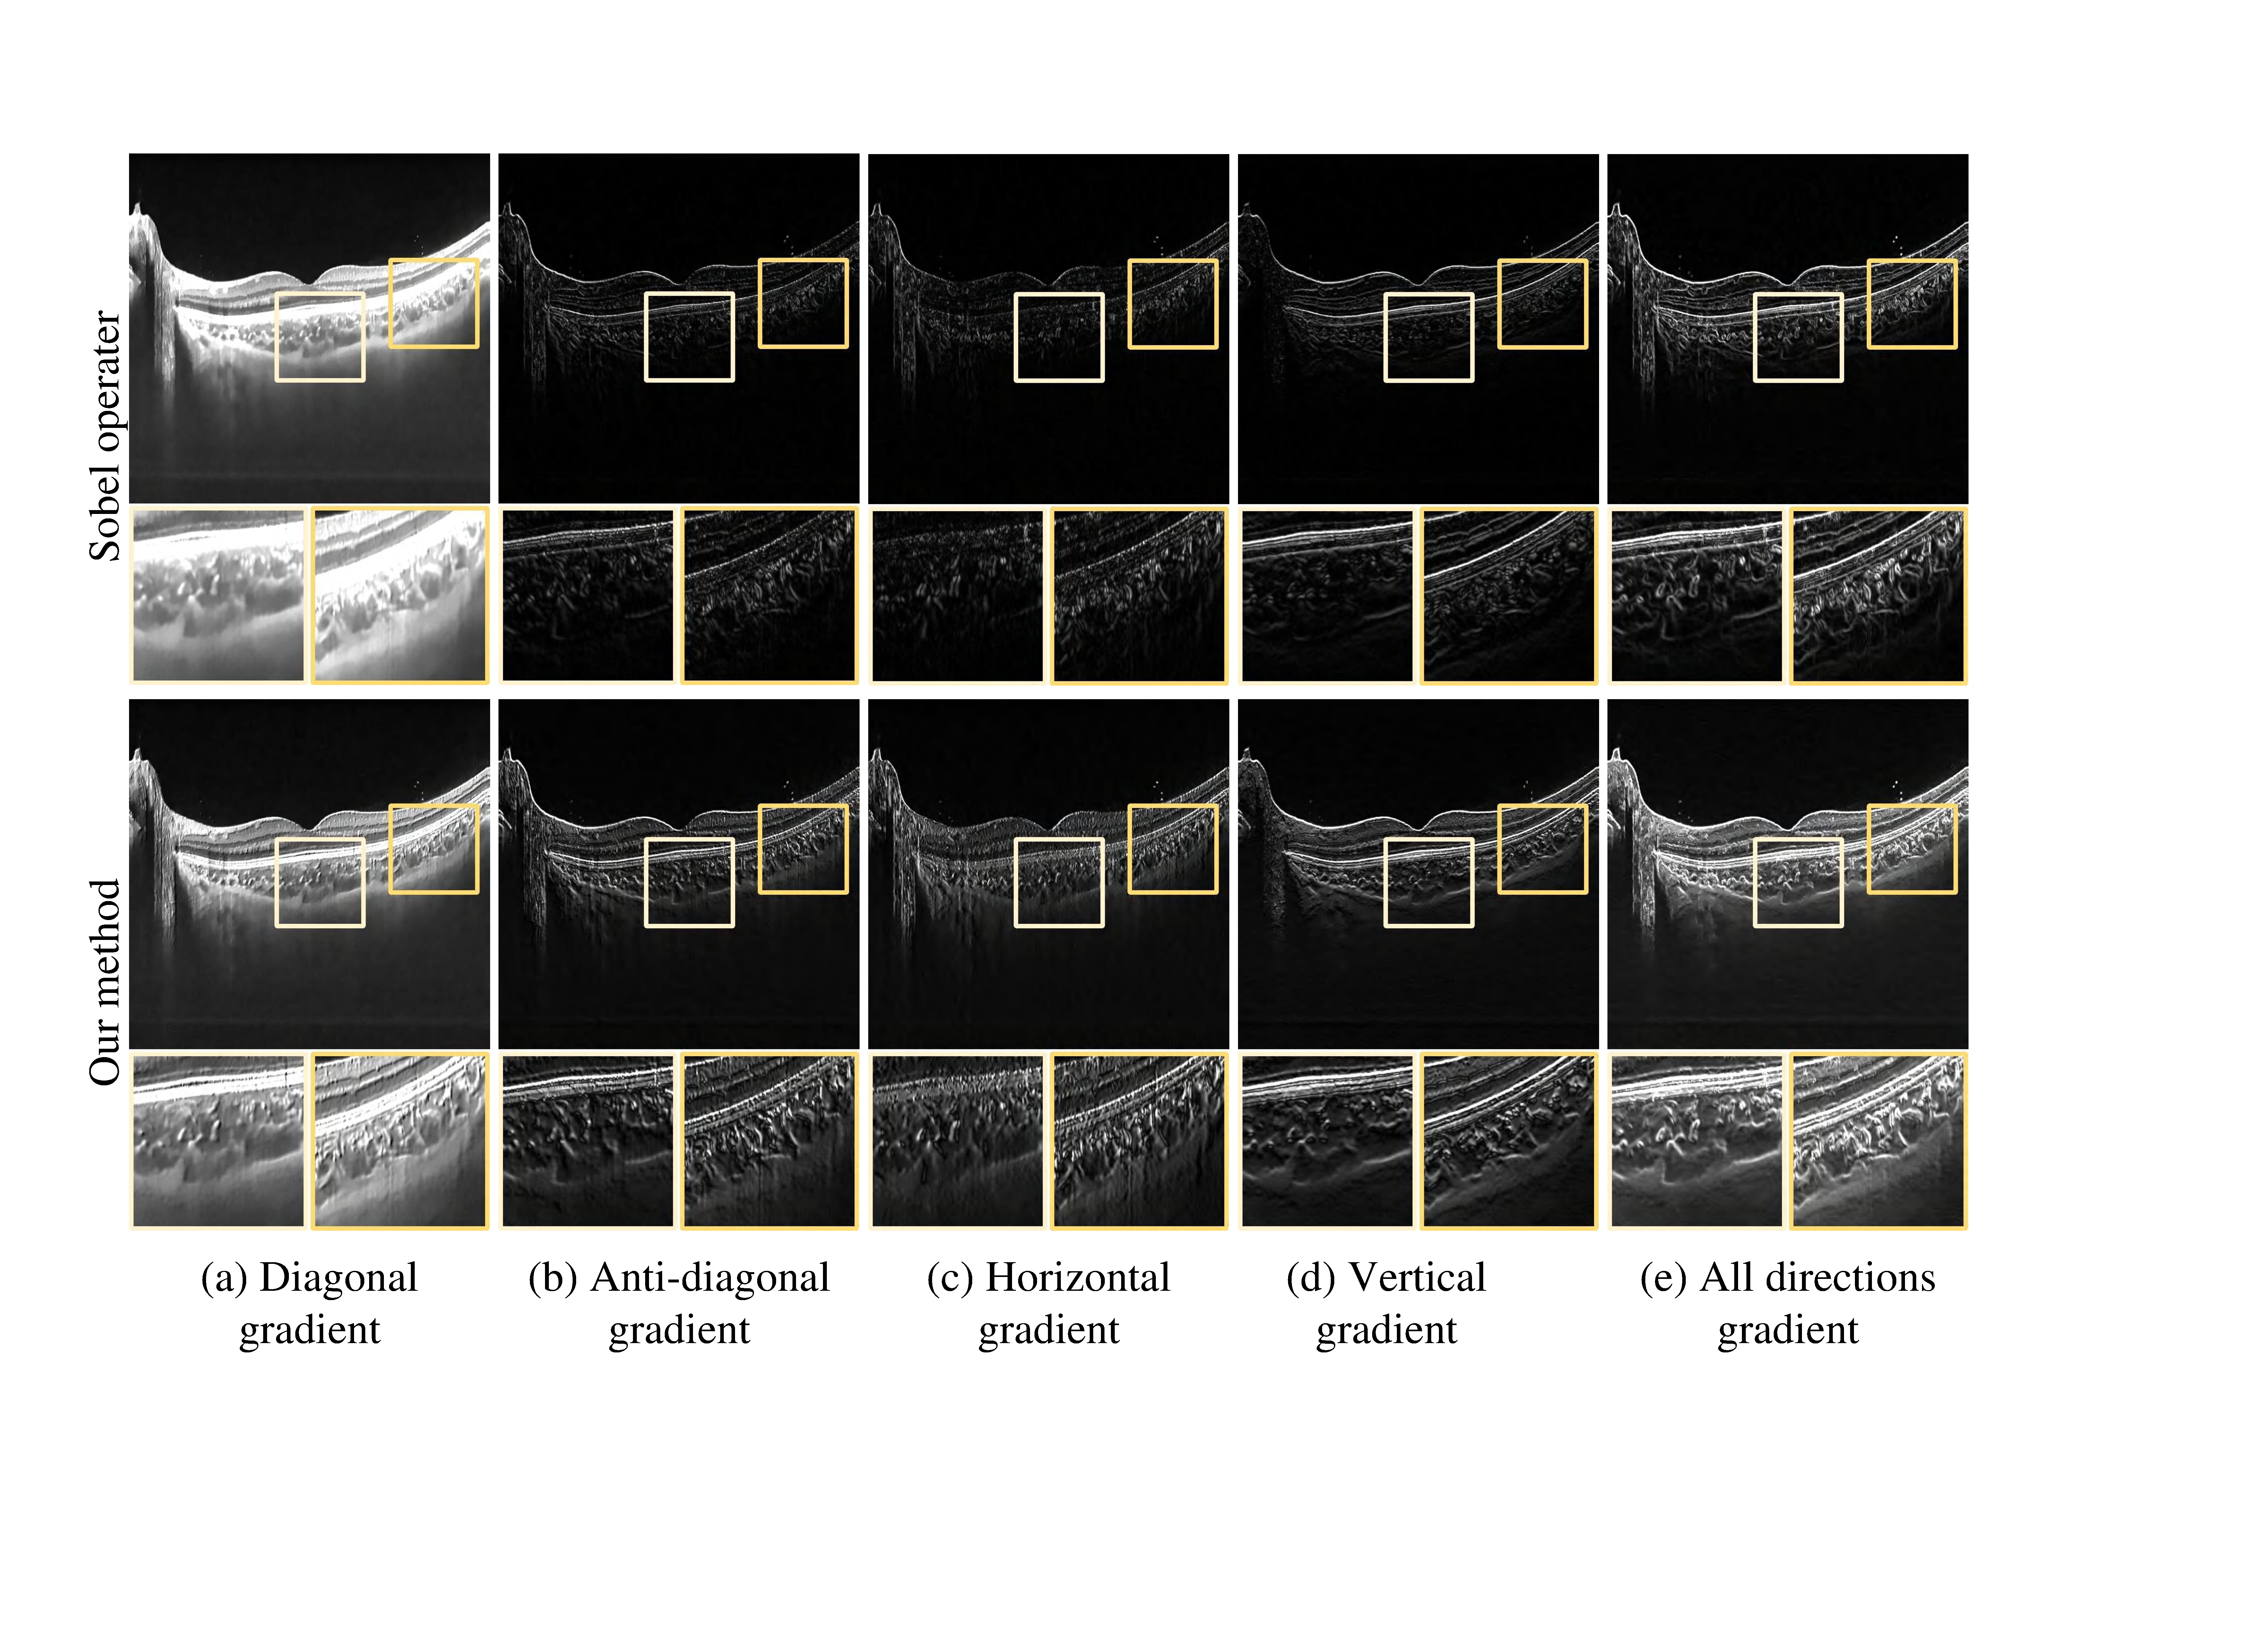
\includegraphics[width=1\linewidth]{fig/edge.pdf}
    \caption{Visual comparison between Sobel edge detection method and our proposed method.
    (a) Diagonal gradient, (b) Anti-diagonal gradient, (c) Horizontal gradient, (d) Vertical gradient, (e) All diretions gradient.
    The first line shows the results of Li \textit{et al}.~\cite{dual_encoder_edge} method, and the second line shows the results of our proposed method.}
    \label{fig:edge_compare}
\end{figure}

\subsection{Refinement Segmentation Stage}
In the refinement stage, dual stem layers partition $x_{\text{masked}}$ and $s_{\text{masked}}$ into non-overlapping $2\times2$ patches, producing feature maps $x'_{\text{masked}}$ and $s'_{\text{masked}}$.
Both image and structure encoders consist of four hierarchical stages with progressive downsampling and channel expansion.
At each stage, a Structure-Aware Module (SAM) fuses OCT image features and UPED-derived structural features to enhance vascular representations.
Multi-scale features are further integrated by the Multi-scale Commingling Attention Module (MCAM), and a joint decoder produces the choroidal layer and vessel predictions $(y_l, y_v)$.
A joint loss function leverages choroidal segmentation to constrain vessel prediction accuracy.

To evaluate scalability, we instantiate SMC-Net with three model sizes, namely SMC-Net-T (Tiny), SMC-Net-S (Small), and SMC-Net-B (Base), with increasing model capacity.At $512\times512$ resolution, SMC-Net is instantiated in three variants: SMC-Net-T has 11.1M parameters and 17.6 GFLOPs, SMC-Net-S has 49.0M parameters and 67.2 GFLOPs, and SMC-Net-B scales to 72.9M parameters with 195.7 GFLOPs.

\subsubsection{SSSD Block}
\begin{figure}[h]
    \centering
    
\includegraphics[width=1\linewidth]{fig/sssd_block.pdf}
    \caption{Visualization of SSSD block composition. (a) SSSD layer, (b) Adaptive Multi-Order Gated Feed-Forward Network (AMG-FFN), (c) SSSD block. A SSSD block consists of a SSSD layer and an AMG-FFN, which are the basic feature extraction blocks of SMC-Net.}
    \label{fig:sssd_block}
\end{figure}

The SSSD block is the fundamental feature extraction unit of SMC-Net, as illustrated in Fig.~\ref{fig:sssd_block}.
It consists of an SSSD layer and an Adaptive Multi-order Gated FFN (AMG-FFN).
Given an input feature map $h \in \mathbb{R}^{H \times W \times C}$, the block is formulated as:
\begin{equation}
\begin{aligned}
h' &= \varPhi_{\text{SSSD}}\!\left(\varPhi_{\text{LN}}(h)\right) + h, \\
z  &= \varPhi_{\text{AMGFFN}}\!\left(\varPhi_{\text{LN}}(h')\right) + h',
\end{aligned}
\label{eq:sssd_block}
\end{equation}
where $\varPhi_{\text{LN}}(\cdot)$ denotes layer normalization, and $z \in \mathbb{R}^{H \times W \times C}$ is the output.
This design follows a Transformer-style residual paradigm, enabling efficient feature modeling for OCT images.

{\color{red} \textbf{(a) SSSD Layer}: To adapt State Space Duality (SSD) to choroidal image segmentation, we propose a Spatiocanal State Space Duality (SSSD) layer that jointly models spatial and inter-channel dependencies.
SSSD employs two complementary streams: a spatial stream for long-range anatomical continuity and a channel stream for modeling correlations among vessel and layer features.
Unlike vanilla SSD, which relies on a single spatial scan and may lose anisotropic boundary cues, SSSD dualizes both dimensions to preserve elongated choroidal structures.
The two streams are processed by parallel Mamba2 blocks~\cite{dao2024transformers} and fused with linear computational complexity, yielding boundary-consistent representations beyond spatial-only state space modeling.}

{\color{red}\textbf{(b) AMG-FFN}: The Adaptive Multi-scale Gated Feed-Forward Network (AMG-FFN) is designed to enhance local feature modeling following the SSSD layer.
Given an input feature map $h$, AMG-FFN extracts multi-scale local features using depth-wise convolutions with different kernel sizes and adaptively fuses them through a gating mechanism:
\begin{equation}
z = \mathcal{F}_{\text{linear}}\big(h \circ \mathcal{G}(\mathcal{F}_{\text{ms}}(h))\big),
\end{equation}
where $\mathcal{F}_{\text{ms}}(\cdot)$ denotes multi-scale depth-wise convolutional feature extraction, $\mathcal{G}(\cdot)$ represents adaptive gating, and $\circ$ is element-wise multiplication.
This design enables AMG-FFN to selectively enhance fine-grained choroidal structures while maintaining computational efficiency.
}

\begin{figure}[h!]
    \centering
    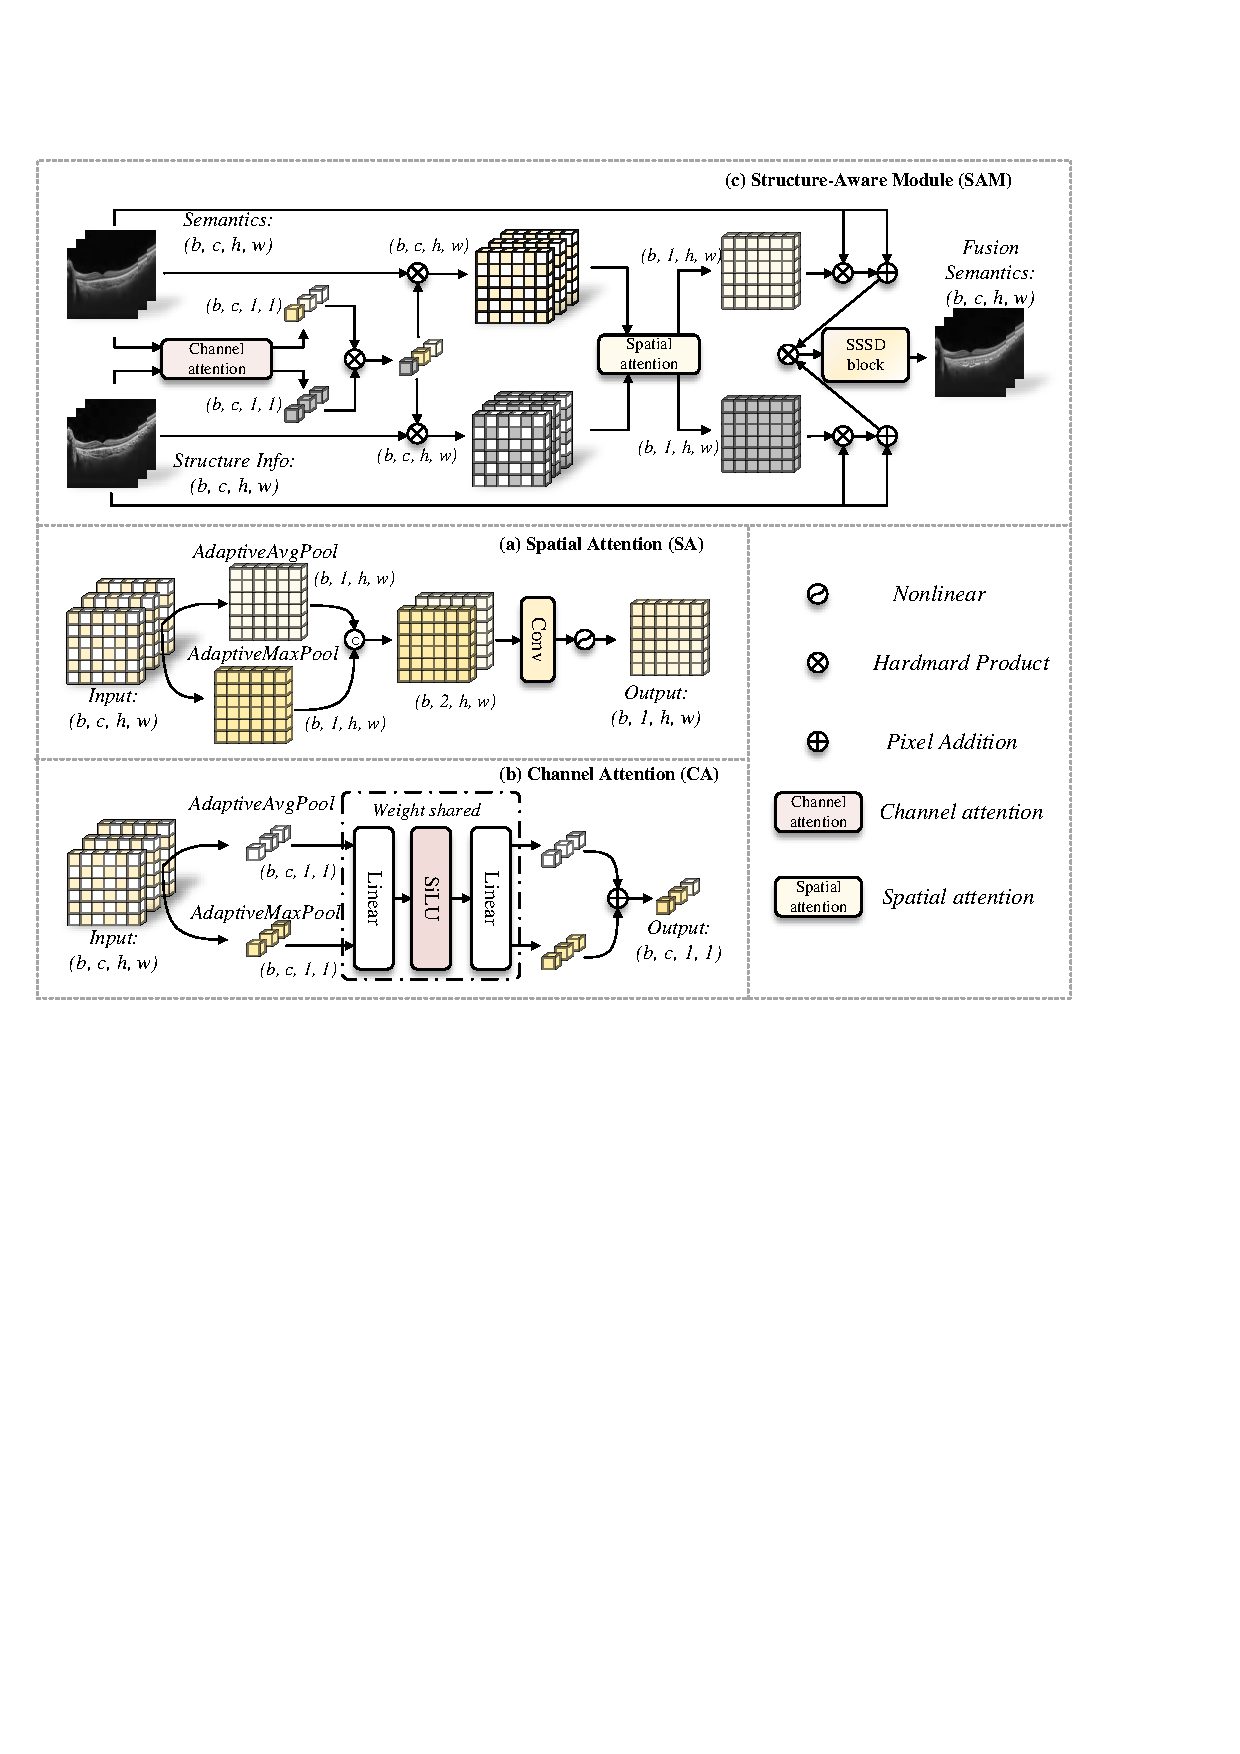
\includegraphics[width=1\linewidth]{fig/sam.pdf}
    \caption{Structure-Aware Module (SAM). SAM integrates semantic features from the OCT image branch with structural cues from the UPED-based structure branch through channel and spatial attention mechanisms.}
    \label{fig:sam}
\end{figure}

\subsubsection{Structure-Aware Module}

{\color{red}
We introduce the Structure-Aware Module (SAM) to fuse semantic features from the OCT encoder with UPED-derived structural cues during refinement (Fig.~\ref{fig:sam}).
SAM injects structural information into semantic representations via channel-wise and spatial attention, enhancing boundary awareness and robustness to OCT noise.
The refined features are then propagated to subsequent SSSD blocks for global modeling.
This lightweight design of SAM sharpens weak vessel boundaries and stabilizes segmentation without noticeable computational overhead.
}

\subsubsection{Multi-Scale Commingling Attention Module}
{\color{red}
To model multi-scale feature interactions more effectively, we propose the Multi-Scale Commingling Attention Module (MCAM), which replaces standard skip-connections in SMC-Net, as illustrated in Fig.~\ref{fig:overview}(d).

MCAM facilitates information exchange across multiple scales between the dual encoders and the decoder, enabling consistent multi-scale representation learning.
Inspired by the skip-connection redesign in U-Net v2~\cite{unetv2}, MCAM integrates channel-wise and spatial attention to recalibrate features at each scale.
MCAM explicitly aligns features from different resolutions and fuses them through multiplicative interaction, emphasizing shared salient structures across scales.
This design is particularly beneficial for joint choroidal layer and vessel modeling, where consistent anatomical cues must be preserved across resolutions.
Specifically, features from different encoder stages are first refined by channel and spatial attention, aligned to a common spatial resolution, and then commingled to produce scale-aware representations.
The fused features are subsequently forwarded to the decoder, enhancing boundary consistency and structural coherence in the final segmentation. MCAM enables consistent multi-scale feature commingling, which is critical for preserving anatomical continuity across resolutions in choroidal segmentation.}

\subsection{Loss Function}
\textbf{Coarse Segmentation Stage}: For the coarse segmentation stage, we adopt a Dice--BCE loss to handle class imbalance and pixel-level variability in medical image segmentation. The $L_{\text{coarse}}$ is defined as:
\begin{align}
L_{\text{Dice}}(y,\hat{y}) &= 1 - \frac{2\sum_{i=1}^{N} y_i \hat{y}_i + \epsilon}{\sum_{i=1}^{N} y_i + \hat{y}_i + \epsilon}, \\
L_{\text{BCE}}(y,\hat{y}) &= -\frac{1}{N}\sum_{i=1}^{N} \big[\hat{y}_i \log(y_i) + (1-\hat{y}_i)\log(1-y_i)\big], \\
L_{\text{coarse}}(y,\hat{y}) &= L_{\text{Dice}}(y,\hat{y}) + L_{\text{BCE}}(y,\hat{y}),
\label{eq:loss_coarse}
\end{align}

where $y$ and $\hat{y}$ denote the prediction and ground truth, respectively, $N$ is the number of pixels, and $\epsilon$ is a smoothing factor.\\
\textbf{Refinement Segmentation Stage}: In the refinement stage, we design a joint loss to simultaneously supervise choroidal layer and vessel segmentation while enforcing anatomical consistency between them.
The joint loss is formulated as:
\begin{equation}
\begin{aligned}
L_{joint}(y,\hat y)&=L_{DiceBCE}(y_v,\hat{y_v})+L_{DiceBCE}(y_l,\hat{y_l})
\\&+\frac{1}{N} \sum_{i=1}^{N} (y_{inter} - \hat{y}_v)^2,
\end{aligned}
\label{eq:loss_refining}
\end{equation}
where $y_v$ and $y_l$ denote the predicted vessel and choroidal layer maps, respectively, $\hat{y}_v$ and $\hat{y}_l$ are the corresponding ground truths, and $y_{\text{inter}} = y_v \cap y_l$ represents the vessel--layer intersection.

{\color{red}
This joint loss explicitly constrains vessel predictions to lie within the choroidal layer, reflecting the anatomical fact that choroidal vessels are embedded inside the layer.
By jointly optimizing $y_l$ and $y_v$, the layer branch provides spatial and boundary guidance for vessel segmentation, effectively suppressing false positives outside the choroid and improving boundary plausibility under severe OCT noise.}

\begin{table*}[!h]
\renewcommand{\arraystretch}{1.1}
\centering
\caption{Comparative experimental results ($mean\pm standard$) of our private OCT-CCV dataset (with \textbf{bold} indicating the best, the \underline{underline} indicates the suboptimal indicators). The indicators include mIoU, DSC, Acc, Spe, and Sen (↑ higher indicators represent better performance of the model). The quantitative results include both the segmentation performance of the choroid layer and the choroidal vessels.}
\label{tab:oct_ccv}
\resizebox{\textwidth}{!}{
\begin{tabular}{@{}llccccclccccc@{}}
\toprule
\multirow{2}{*}{\textbf{Dataset}} & \multirow{2}{*}{\textbf{Model}} & \textbf{mloU(\%)↑} & \textbf{DSC(\%)↑} & \textbf{Acc(\%)↑} & \textbf{Spe(\%)↑} & \textbf{Sen(\%)↑} &  & \textbf{mloU(\%)↑} & \textbf{DSC(\%)↑} & \textbf{Acc(\%)↑} & \textbf{Spe(\%)↑} & \textbf{Sen(\%)↑} \\ \cmidrule(lr){3-7} \cmidrule(l){9-13} 
 &  & \multicolumn{5}{c}{Segmentation Objects: Choroidal Layer} &  & \multicolumn{5}{c}{Segmentation Objects: Choroidal Vessel} \\ \midrule
\multirow{17}{*}{OCT-CCV} & UNet~\cite{ronneberger2015u} & $94.43 \pm 0.21$ & $97.13 \pm 0.15$ & $99.57 \pm 0.05$ & $99.72 \pm 0.04$ & $97.78 \pm 0.18$ &  & $40.29 \pm 0.20$ & $57.44 \pm 0.31$ & $97.56 \pm 0.08$ & $98.72 \pm 0.06$ & $57.83 \pm 0.29$ \\
 & {\color{red}nnU-Net~\cite{Isensee2021}} & {\color{red}$94.70 \pm 0.18$} & {\color{red}$97.25 \pm 0.14$} & {\color{red}$99.60 \pm 0.05$} & {\color{red}$99.74 \pm 0.04$} & {\color{red}$97.85 \pm 0.16$} &  & {\color{red}$45.10 \pm 0.22$} & {\color{red}$61.50 \pm 0.28$} & {\color{red}$97.70 \pm 0.09$} & {\color{red}$98.90 \pm 0.06$} & {\color{red}$62.00 \pm 0.25$} \\
 & AttnUNet~\cite{Oktay2018AttentionUNet} & $94.29 \pm 0.22$ & $97.06 \pm 0.17$ & $99.56 \pm 0.06$ & $99.70 \pm 0.03$ & $97.76 \pm 0.19$ &  & $46.00 \pm 0.18$ & $63.01 \pm 0.23$ & $97.85 \pm 0.07$ & $98.84 \pm 0.04$ & $62.27 \pm 0.19$ \\
 & R2UNet~\cite{alom2018recurrentresidualconvolutionalneural} & $-$ & $0.0 \pm 0.0$ & $92.61 \pm 0.10$ & $1.0 \pm 0.0$ & $0.0 \pm 0.0$ &  & $-$ & $0.0 \pm 0.0$ & $97.16 \pm 0.09$ & $1.0 \pm 0.0$ & $0.0 \pm 0.0$ \\
 & R2AUNet~\cite{R2AU-Net} & $-$ & $0.0 \pm 0.0$ & $92.61 \pm 0.11$ & $1.0 \pm 0.0$ & $0.0 \pm 0.0$ &  & $-$ & $0.0 \pm 0.0$ & $97.15 \pm 0.08$ & $1.0 \pm 0.0$ & $0.0 \pm 0.0$ \\
 & UNetV2~\cite{unetv2} & $94.61 \pm 0.25$ & $97.35 \pm 0.19$ & $99.61 \pm 0.04$ & $99.77 \pm 0.02$ & $97.79 \pm 0.17$ &  & $52.41 \pm 0.21$ & $69.74 \pm 0.18$ & $97.96 \pm 0.09$ & $98.92 \pm 0.05$ & $67.43 \pm 0.26$ \\
 & MALUNet~\cite{ruan2022malunet} & $95.11 \pm 0.18$ & $97.49 \pm 0.12$ & $99.63 \pm 0.05$ & $99.79 \pm 0.02$ & $97.59 \pm 0.14$ &  & $22.46 \pm 0.15$ & $36.68 \pm 0.23$ & $96.50 \pm 0.10$ & $98.28 \pm 0.08$ & $35.68 \pm 0.21$ \\
 & H-vmunet~\cite{wu2024hvmunethighordervisionmamba} & $94.75 \pm 0.20$ & $97.31 \pm 0.16$ & $99.60 \pm 0.05$ & $99.75 \pm 0.03$ & $97.68 \pm 0.17$ &  & $31.52 \pm 0.19$ & $47.93 \pm 0.21$ & $97.40 \pm 0.09$ & $99.02 \pm 0.04$ & $42.09 \pm 0.22$ \\
 & UL-vmunet~\cite{wu2024ultralightvmunetparallelvision} & $92.55 \pm 0.23$ & $96.13 \pm 0.21$ & $99.42 \pm 0.07$ & $99.65 \pm 0.04$ & $96.55 \pm 0.14$ &  & $27.38 \pm 0.20$ & $42.99 \pm 0.22$ & $97.09 \pm 0.10$ & $98.80 \pm 0.05$ & $38.55 \pm 0.18$ \\
 & VM-UNet~\cite{vmunet} & $97.16 \pm 0.17$ & $98.56 \pm 0.12$ & $99.79 \pm 0.05$ & $99.87 \pm 0.02$ & $98.78 \pm 0.09$ &  & $38.07 \pm 0.21$ & $55.15 \pm 0.14$ & $97.49 \pm 0.08$ & $98.76 \pm 0.04$ & $54.23 \pm 0.16$ \\
 & VM-UNetV2~\cite{vmunetv2} & $97.71 \pm 0.14$ & $98.85 \pm 0.11$ & \underline{$99.83 \pm 0.06$} & \underline{$99.90 \pm 0.01$} & \underline{$98.98 \pm 0.08$} &  & $41.19 \pm 0.18$ & $58.34 \pm 0.15$ & $97.95 \pm 0.07$ & $99.33 \pm 0.03$ & $50.60 \pm 0.12$ \\
 & CVI-Net~\cite{cvinet} & $89.83 \pm 0.28$ & $94.66 \pm 0.22$ & $99.18 \pm 0.09$ & $99.31 \pm 0.04$ & $97.58 \pm 0.16$ &  & $23.76 \pm 0.24$ & $38.40 \pm 0.27$ & $95.95 \pm 0.11$ & $97.46 \pm 0.06$ & $44.39 \pm 0.21$ \\
 & ChoroidNET~\cite{choroidnet} & $94.82 \pm 0.19$ & $97.34 \pm 0.14$ & $99.60 \pm 0.04$ & $99.70 \pm 0.03$ & $97.89 \pm 0.15$ &  & $62.26 \pm 0.54$ & $76.74 \pm 0.74$ & $98.55 \pm 0.08$ & $98.96 \pm 0.04$ & $84.29 \pm 0.10$ \\
 & TACLNet~\cite{wen2024} & $95.06 \pm 0.20$ & $97.43 \pm 0.13$ & $99.57 \pm 0.05$ & $99.74 \pm 0.03$ & $97.97 \pm 0.17$ &  & \underline{$75.21 \pm 0.22$} & \underline{$86.30 \pm 0.27$} & \underline{$99.21 \pm 0.06$} & \underline{$99.31 \pm 0.02$} & \underline{$84.65 \pm 0.12$} \\ \cmidrule(lr){2-7} \cmidrule(l){9-13} 
 & SMC-Net-T (ours) & $95.10 \pm 0.18$ & $97.60 \pm 0.12$ & $99.61 \pm 0.05$ & $99.76 \pm 0.02$ & $97.80 \pm 0.16$ &  & $70.19 \pm 0.21$ & $78.26 \pm 0.24$ & $98.67 \pm 0.07$ & $98.51 \pm 0.04$ & $83.58 \pm 0.15$ \\
 & SMC-Net-S (ours) & \boldmath$99.80 \pm 0.10$ & \boldmath$99.89 \pm 0.07$ & \boldmath$99.87 \pm 0.04$ & \boldmath$99.91 \pm 0.03$ & \boldmath$99.79 \pm 0.03$ &  & \boldmath$75.58 \pm 0.19$ & \boldmath$86.40 \pm 0.22$ & \boldmath$99.30 \pm 0.08$ & \boldmath$99.64 \pm 0.02$ & \boldmath$84.83 \pm 0.11$ \\
 & SMC-Net-B (ours) & \underline{$99.65 \pm 0.11$} & \underline{$99.74 \pm 0.08$} & $99.74 \pm 0.06$ & $99.71 \pm 0.02$ & $97.84 \pm 0.14$ &  & $75.20 \pm 0.21$ & $86.25 \pm 0.23$ & $99.20 \pm 0.09$ & \underline{$99.31 \pm 0.04$} & $84.59 \pm 0.12$ \\ \bottomrule
\end{tabular}
}
\end{table*}

\begin{table*}[!h]
\renewcommand{\arraystretch}{1.1}
\centering
\caption{Comparative experimental results ($mean\pm standard$) of RETOUCH dataset~\cite{RETOUCH} (with \textbf{bold} indicating the best, the \underline{underline} indicates the suboptimal indicators). The indicators include mIoU, DSC, Acc, Spe, and Sen (↑ higher indicators represent better performance of the model). The quantitative results include both the segmentation performance of the retinal layer and the fluids.}
\label{tab:retouch}
\resizebox{\textwidth}{!}{
\begin{tabular}{@{}llccccclccccc@{}}
\toprule
\multirow{2}{*}{\textbf{Dataset}} & \multirow{2}{*}{\textbf{Model}} & \textbf{mloU(\%)↑} & \textbf{DSC(\%)↑} & \textbf{Acc(\%)↑} & \textbf{Spe(\%)↑} & \textbf{Sen(\%)↑} &  & \textbf{mloU(\%)↑} & \textbf{DSC(\%)↑} & \textbf{Acc(\%)↑} & \textbf{Spe(\%)↑} & \textbf{Sen(\%)↑} \\ \cmidrule(lr){3-7} \cmidrule(l){9-13} 
 &  & \multicolumn{5}{c}{Segmentation Objects: Retinal Layer} &  & \multicolumn{5}{c}{Segmentation Objects: Fluids} \\ \midrule
\multirow{16}{*}{\begin{tabular}[c]{@{}l@{}}RETOUCH\\ ~\cite{RETOUCH}\end{tabular}} & UNet~\cite{ronneberger2015u} & $98.19 \pm 0.10$ & $99.01 \pm 0.07$ & $99.58 \pm 0.12$ & $99.68 \pm 0.05$ & \boldmath{$99.17 \pm 0.06$} &  & $37.70 \pm 0.30$ & $54.75 \pm 0.25$ & $96.79 \pm 0.15$ & $97.41 \pm 0.10$ & $73.66 \pm 0.20$ \\
 & {\color{red}nnU-Net~\cite{Isensee2021}} & {\color{red}$98.25 \pm 0.09$} & {\color{red}$99.05 \pm 0.06$} & {\color{red}$99.59 \pm 0.11$} & {\color{red}$99.69 \pm 0.05$} & {\color{red}$99.12 \pm 0.06$} &  & {\color{red}$38.50 \pm 0.28$} & {\color{red}$55.50 \pm 0.24$} & {\color{red}$96.90 \pm 0.13$} & {\color{red}$97.50 \pm 0.09$} & {\color{red}$74.20 \pm 0.19$} \\
 & AttnUNet~\cite{Oktay2018AttentionUNet} & $98.28 \pm 0.08$ & $99.08 \pm 0.06$ & $99.57 \pm 0.09$ & $99.68 \pm 0.04$ & \underline{$99.16 \pm 0.05$} &  & $35.59 \pm 0.32$ & $52.49 \pm 0.29$ & $96.38 \pm 0.18$ & $96.95 \pm 0.12$ & $75.72 \pm 0.18$ \\
 & R2UNet~\cite{alom2018recurrentresidualconvolutionalneural} & $0.00 \pm 0.00$ & $0.00 \pm 0.00$ & $79.90 \pm 0.10$ & $1.00 \pm 0.00$ & $0.00 \pm 0.00$ &  & $22.57 \pm 0.34$ & $36.82 \pm 0.25$ & $95.03 \pm 0.12$ & $96.11 \pm 0.08$ & $54.97 \pm 0.15$ \\
 & R2AUNet~\cite{R2AU-Net} & $50.08 \pm 0.25$ & $66.74 \pm 0.20$ & $88.84 \pm 0.14$ & $97.17 \pm 0.05$ & $55.72 \pm 0.13$ &  & $0.00 \pm 0.00$ & $0.00 \pm 0.00$ & $97.36 \pm 0.10$ & $1.00 \pm 0.00$ & $0.00 \pm 0.00$ \\
 & UNetV2~\cite{unetv2} & $97.74 \pm 0.15$ & $98.86 \pm 0.10$ & $99.54 \pm 0.08$ & $99.70 \pm 0.03$ & $98.90 \pm 0.05$ &  & $11.01 \pm 0.25$ & $19.84 \pm 0.18$ & $88.80 \pm 0.20$ & $89.79 \pm 0.12$ & $52.53 \pm 0.16$ \\
 & MALUNet~\cite{ruan2022malunet} & $97.86 \pm 0.12$ & $98.92 \pm 0.08$ & $99.57 \pm 0.09$ & $99.72 \pm 0.04$ & $98.95 \pm 0.06$ &  & $24.42 \pm 0.30$ & $39.25 \pm 0.25$ & $94.89 \pm 0.16$ & $95.76 \pm 0.11$ & $62.61 \pm 0.14$ \\
 & H-vmunet~\cite{wu2024hvmunethighordervisionmamba} & $98.14 \pm 0.11$ & $99.06 \pm 0.07$ & $99.62 \pm 0.10$ & $99.75 \pm 0.04$ & $99.13 \pm 0.06$ &  & $28.66 \pm 0.25$ & $44.56 \pm 0.22$ & $95.69 \pm 0.13$ & $96.50 \pm 0.09$ & $65.65 \pm 0.12$ \\
 & UL-vmunet~\cite{wu2024ultralightvmunetparallelvision} & $97.61 \pm 0.14$ & $98.79 \pm 0.09$ & $99.51 \pm 0.11$ & $99.64 \pm 0.04$ & $99.00 \pm 0.07$ &  & $29.36 \pm 0.23$ & $45.39 \pm 0.20$ & $95.36 \pm 0.14$ & $95.97 \pm 0.08$ & $73.05 \pm 0.10$ \\
 & VM-UNet~\cite{vmunet} & $98.27 \pm 0.09$ & $99.13 \pm 0.06$ & $99.65 \pm 0.08$ & $99.78 \pm 0.03$ & $99.13 \pm 0.05$ &  & $39.86 \pm 0.22$ & $56.99 \pm 0.19$ & $96.76 \pm 0.12$ & $97.17 \pm 0.07$ & $81.43 \pm 0.13$ \\
 & VM-UNetV2~\cite{vmunetv2} & $98.18 \pm 0.10$ & $99.08 \pm 0.07$ & $99.63 \pm 0.09$ & $99.76 \pm 0.03$ & $99.10 \pm 0.06$ &  & $35.39 \pm 0.27$ & $52.28 \pm 0.23$ & $97.00 \pm 0.15$ & $97.92 \pm 0.08$ & $62.53 \pm 0.14$ \\
 & ChoroidNET~\cite{choroidnet} & $98.20 \pm 0.11$ & $99.04 \pm 0.08$ & $99.59 \pm 0.10$ & $99.67 \pm 0.03$ & $99.15 \pm 0.05$ &  & $48.10 \pm 0.18$ & $64.96 \pm 0.17$ & $98.15 \pm 0.09$ & $99.06 \pm 0.05$ & $64.72 \pm 0.12$ \\
 & TACLNet~\cite{wen2024} & \underline{$98.39 \pm 0.08$} & \underline{$99.19 \pm 0.06$} & \underline{$99.66 \pm 0.07$} & $99.77 \pm 0.03$ & $99.14 \pm 0.05$ &  & $71.10 \pm 0.21$ & $83.11 \pm 0.18$ & $99.10 \pm 0.10$ & $99.54 \pm 0.06$ & $83.31 \pm 0.11$ \\ \cmidrule(l){2-13} 
 & SMC-Net-T (ours) & $97.69 \pm 0.10$ & $98.88 \pm 0.07$ & $99.54 \pm 0.11$ & $99.68 \pm 0.03$ & $98.97 \pm 0.05$ &  & $69.55 \pm 0.19$ & $78.85 \pm 0.16$ & $98.66 \pm 0.14$ & $98.41 \pm 0.08$ & $80.51 \pm 0.13$ \\
 & SMC-Net-S (ours) & \boldmath{$98.40 \pm 0.09$} & \boldmath{$99.20 \pm 0.06$} & \boldmath{$99.68 \pm 0.08$} & \boldmath{$99.81 \pm 0.03$} & \boldmath{$99.17 \pm 0.05$} &  & \boldmath{$73.70 \pm 0.20$} & \boldmath{$84.86 \pm 0.17$} & \boldmath{$99.20 \pm 0.12$} & \boldmath{$99.60 \pm 0.07$} & \boldmath{$84.76 \pm 0.11$} \\
 & SMC-Net-B (ours) & $98.37 \pm 0.10$ & $99.16 \pm 0.07$ & $99.64 \pm 0.09$ & \underline{$99.79 \pm 0.03$} & $99.14 \pm 0.05$ &  & \underline{$73.65 \pm 0.19$} & \underline{$84.80 \pm 0.16$} & \underline{$99.18 \pm 0.11$} & \underline{$99.55 \pm 0.07$} & \underline{$84.70 \pm 0.12$} \\ \bottomrule
\end{tabular}
}
\end{table*}

\section{Experiments}
\subsection{Dataset}
\textbf{OCT Clinical Choroidal Vessel Dataset (OCT-CCV)}: {\color{red}All OCT-CCV images used in this study were retrospectively collected at Shanghai General Hospital, Shanghai Jiao Tong University, between 2023 and 2024. The data collection was conducted under the approval of the institutional review board and in accordance with the Declaration of Helsinki. Informed consent was waived due to the retrospective study design and use of anonymized
data.}
This dataset consists of 120 images collected by experienced ophthalmologists using swept-source OCT. Each image is averaged from 32 overlapping scans centered on the fovea, with a resolution of $1024\times992$. Ten subjects (five emmetropic and five highly myopic, $\leqslant -5.0$) were randomly selected. Two ophthalmologists independently annotated the choroid layer and vessels, followed by joint verification. We use 5-fold cross-validation for evaluation: in each fold, eight studies (96 images, $\sim$8,740 annotated regions, resized to $512\times512$) form the training set, while the remaining two studies (24 images, $\sim$2,190 regions) form the test set.


\textbf{RETOUCH Dataset}: To demonstrate SMC-Net's generalization across medical segmentation tasks, we evaluated it on the public RETOUCH~\cite{RETOUCH} dataset for segmenting retinal edema. RETOUCH contains three training sets from different OCT devices, totaling 70 volumes. Following a 5-fold cross-validation at the case level, we labeled the retina layer for training. Specifically, 711 slices from 24 SD-OCT volumes acquired with the Spectralis device (Heidelberg) were randomly selected. These slices already contain official fluid labels, and the retinal layer was further annotated and verified by two experienced doctors.

\begin{figure*}[!ht]
    \centering
    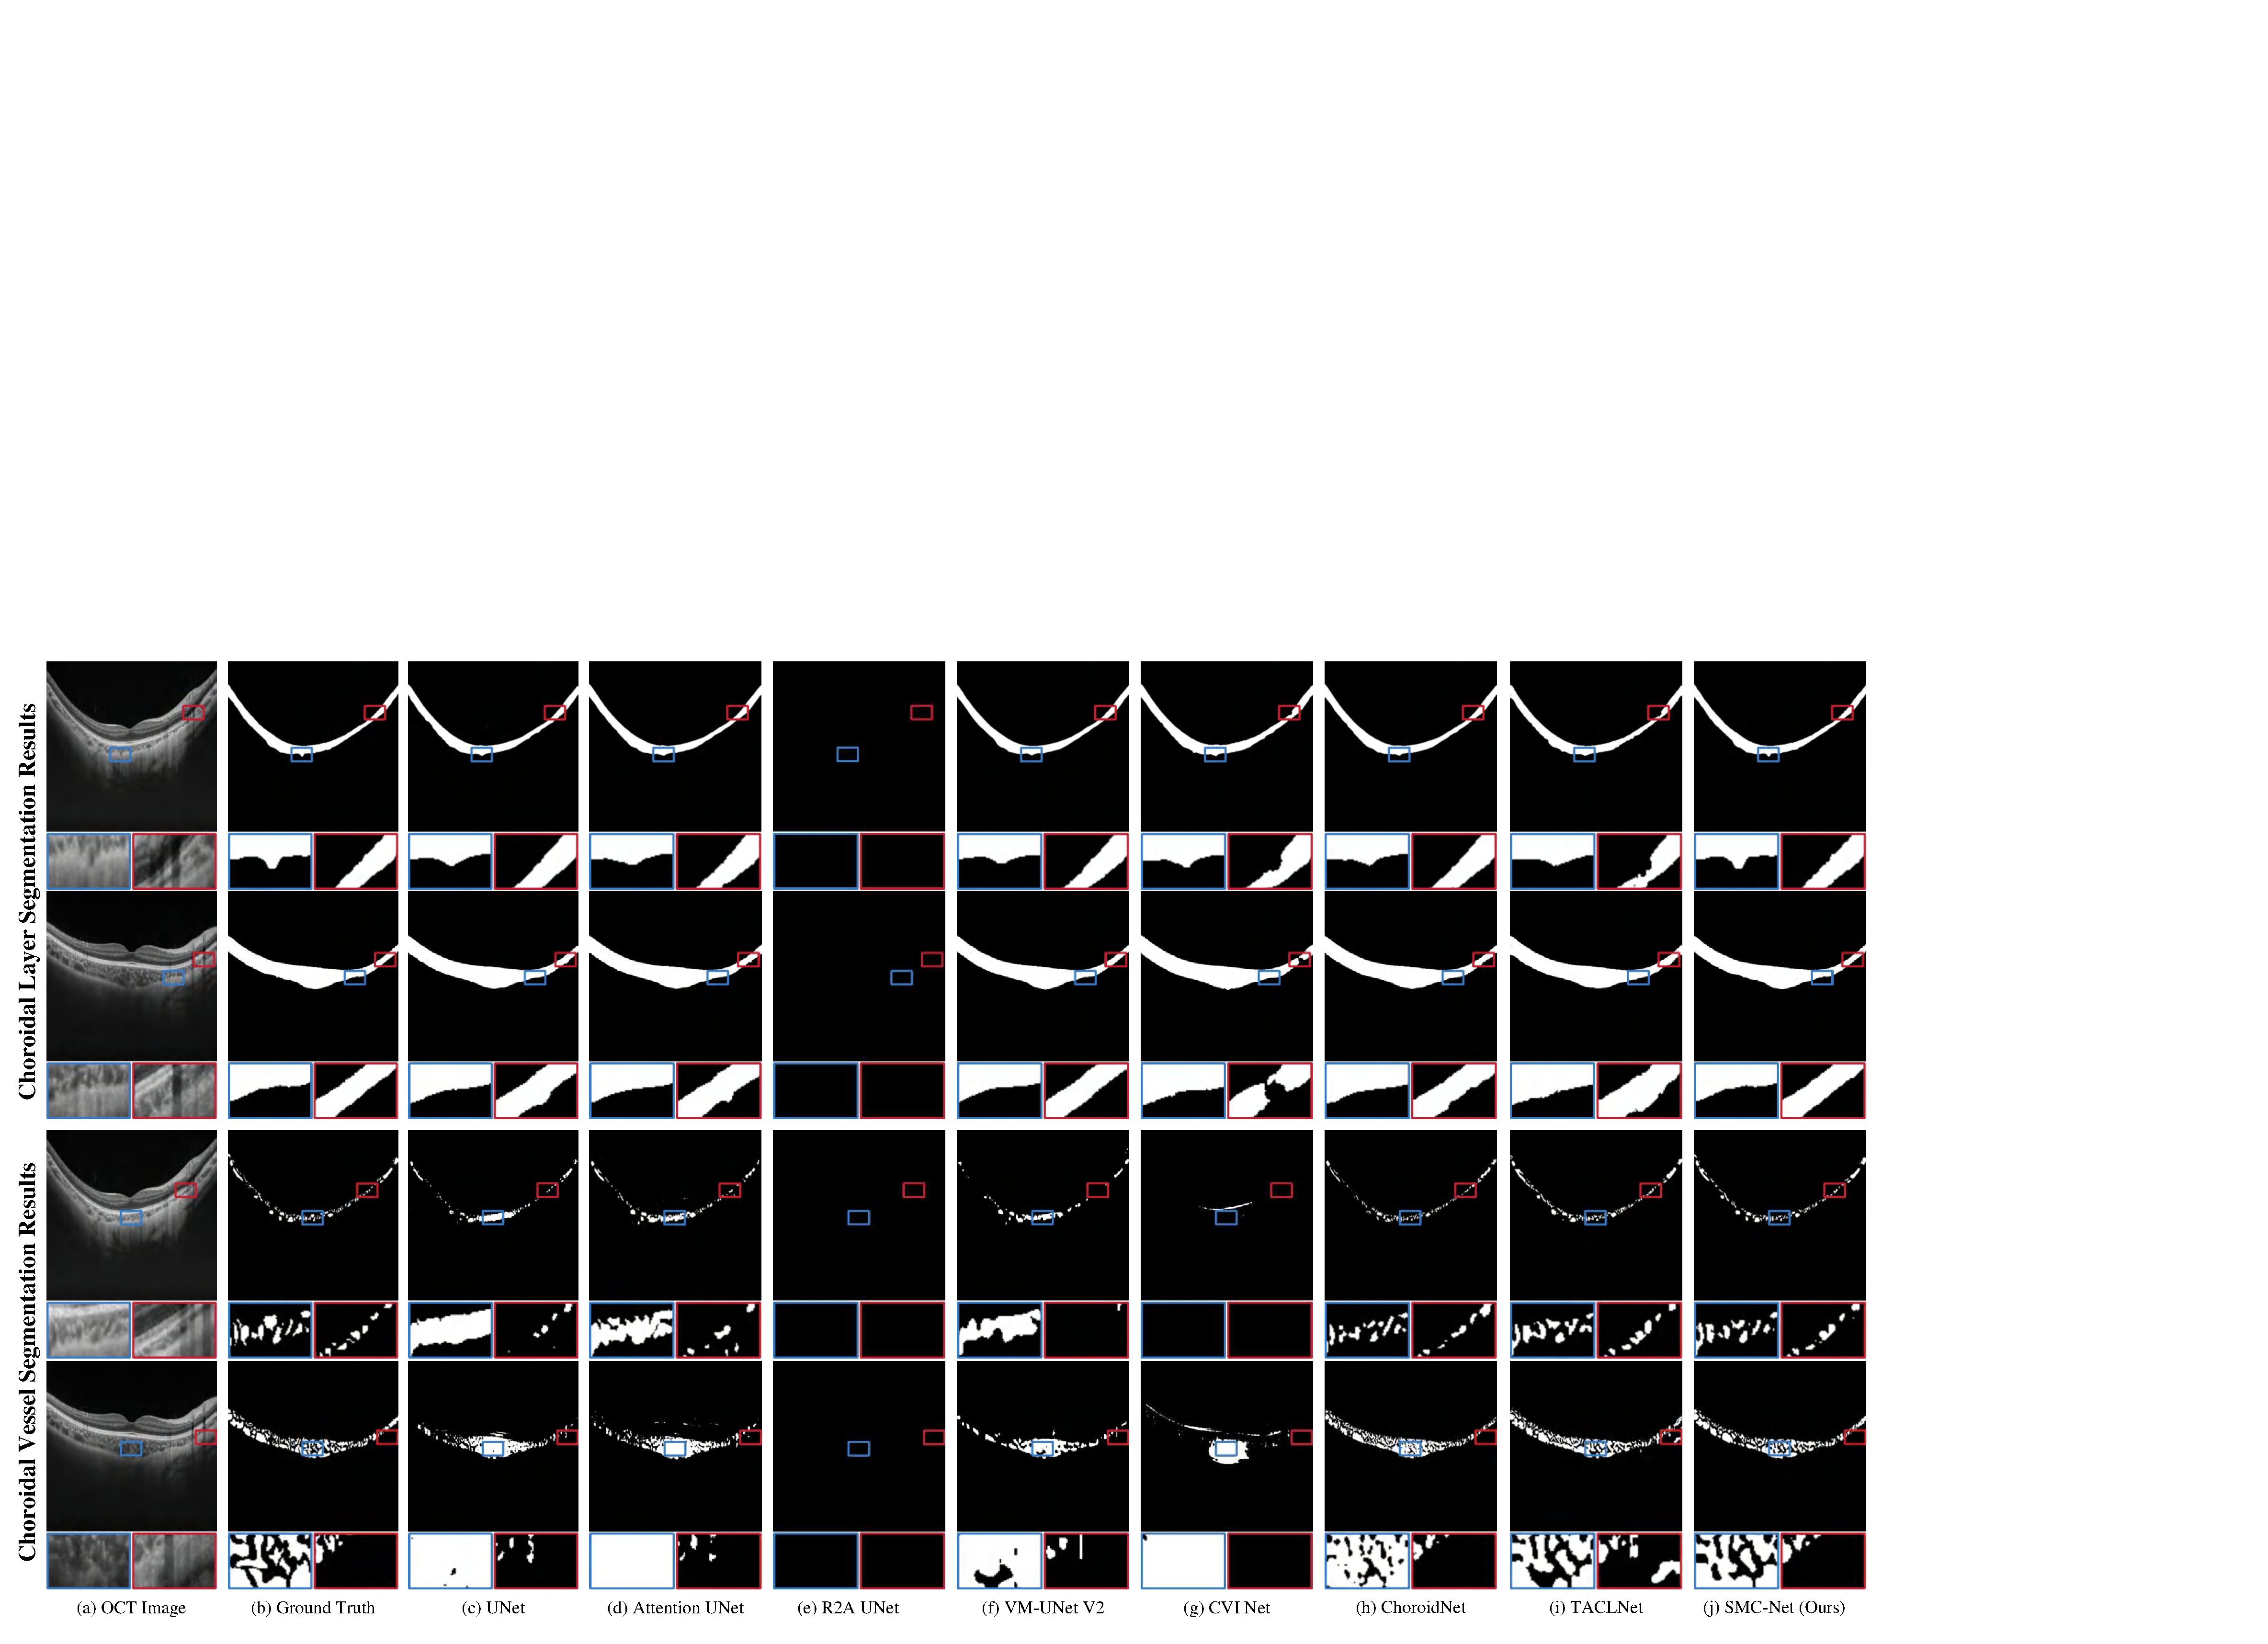
\includegraphics[width=0.9\linewidth]{fig/resultsOctccv.pdf}
    \caption{Qualitative visualization on the private dataset OCT-CCV. The top two rows show the segmentation visualizations for the choroid layer, and the bottom two rows show the segmentation visualizations for the choroid vessels. (a) OCT image, (b) Ground Truth, (c) UNet~\cite{ronneberger2015u}, (d) Attention UNet~\cite{Oktay2018AttentionUNet}, (e) R2A UNet~\cite{R2AU-Net}, (f) VM-UNet V2~\cite{vmunetv2}, (g) CVI Net~\cite{cvinet}, (h) ChoroidNet~\cite{choroidnet}, (i) TACLNet~\cite{wen2024}, (j) SMC-Net (Ours). Below each image, a zoomed-in view of the highlighted area (red and blue boxes) is provided to facilitate the observation of differences.}
    \label{fig:resultsOctccv}
\end{figure*}
\begin{figure*}[!ht]
    \centering
    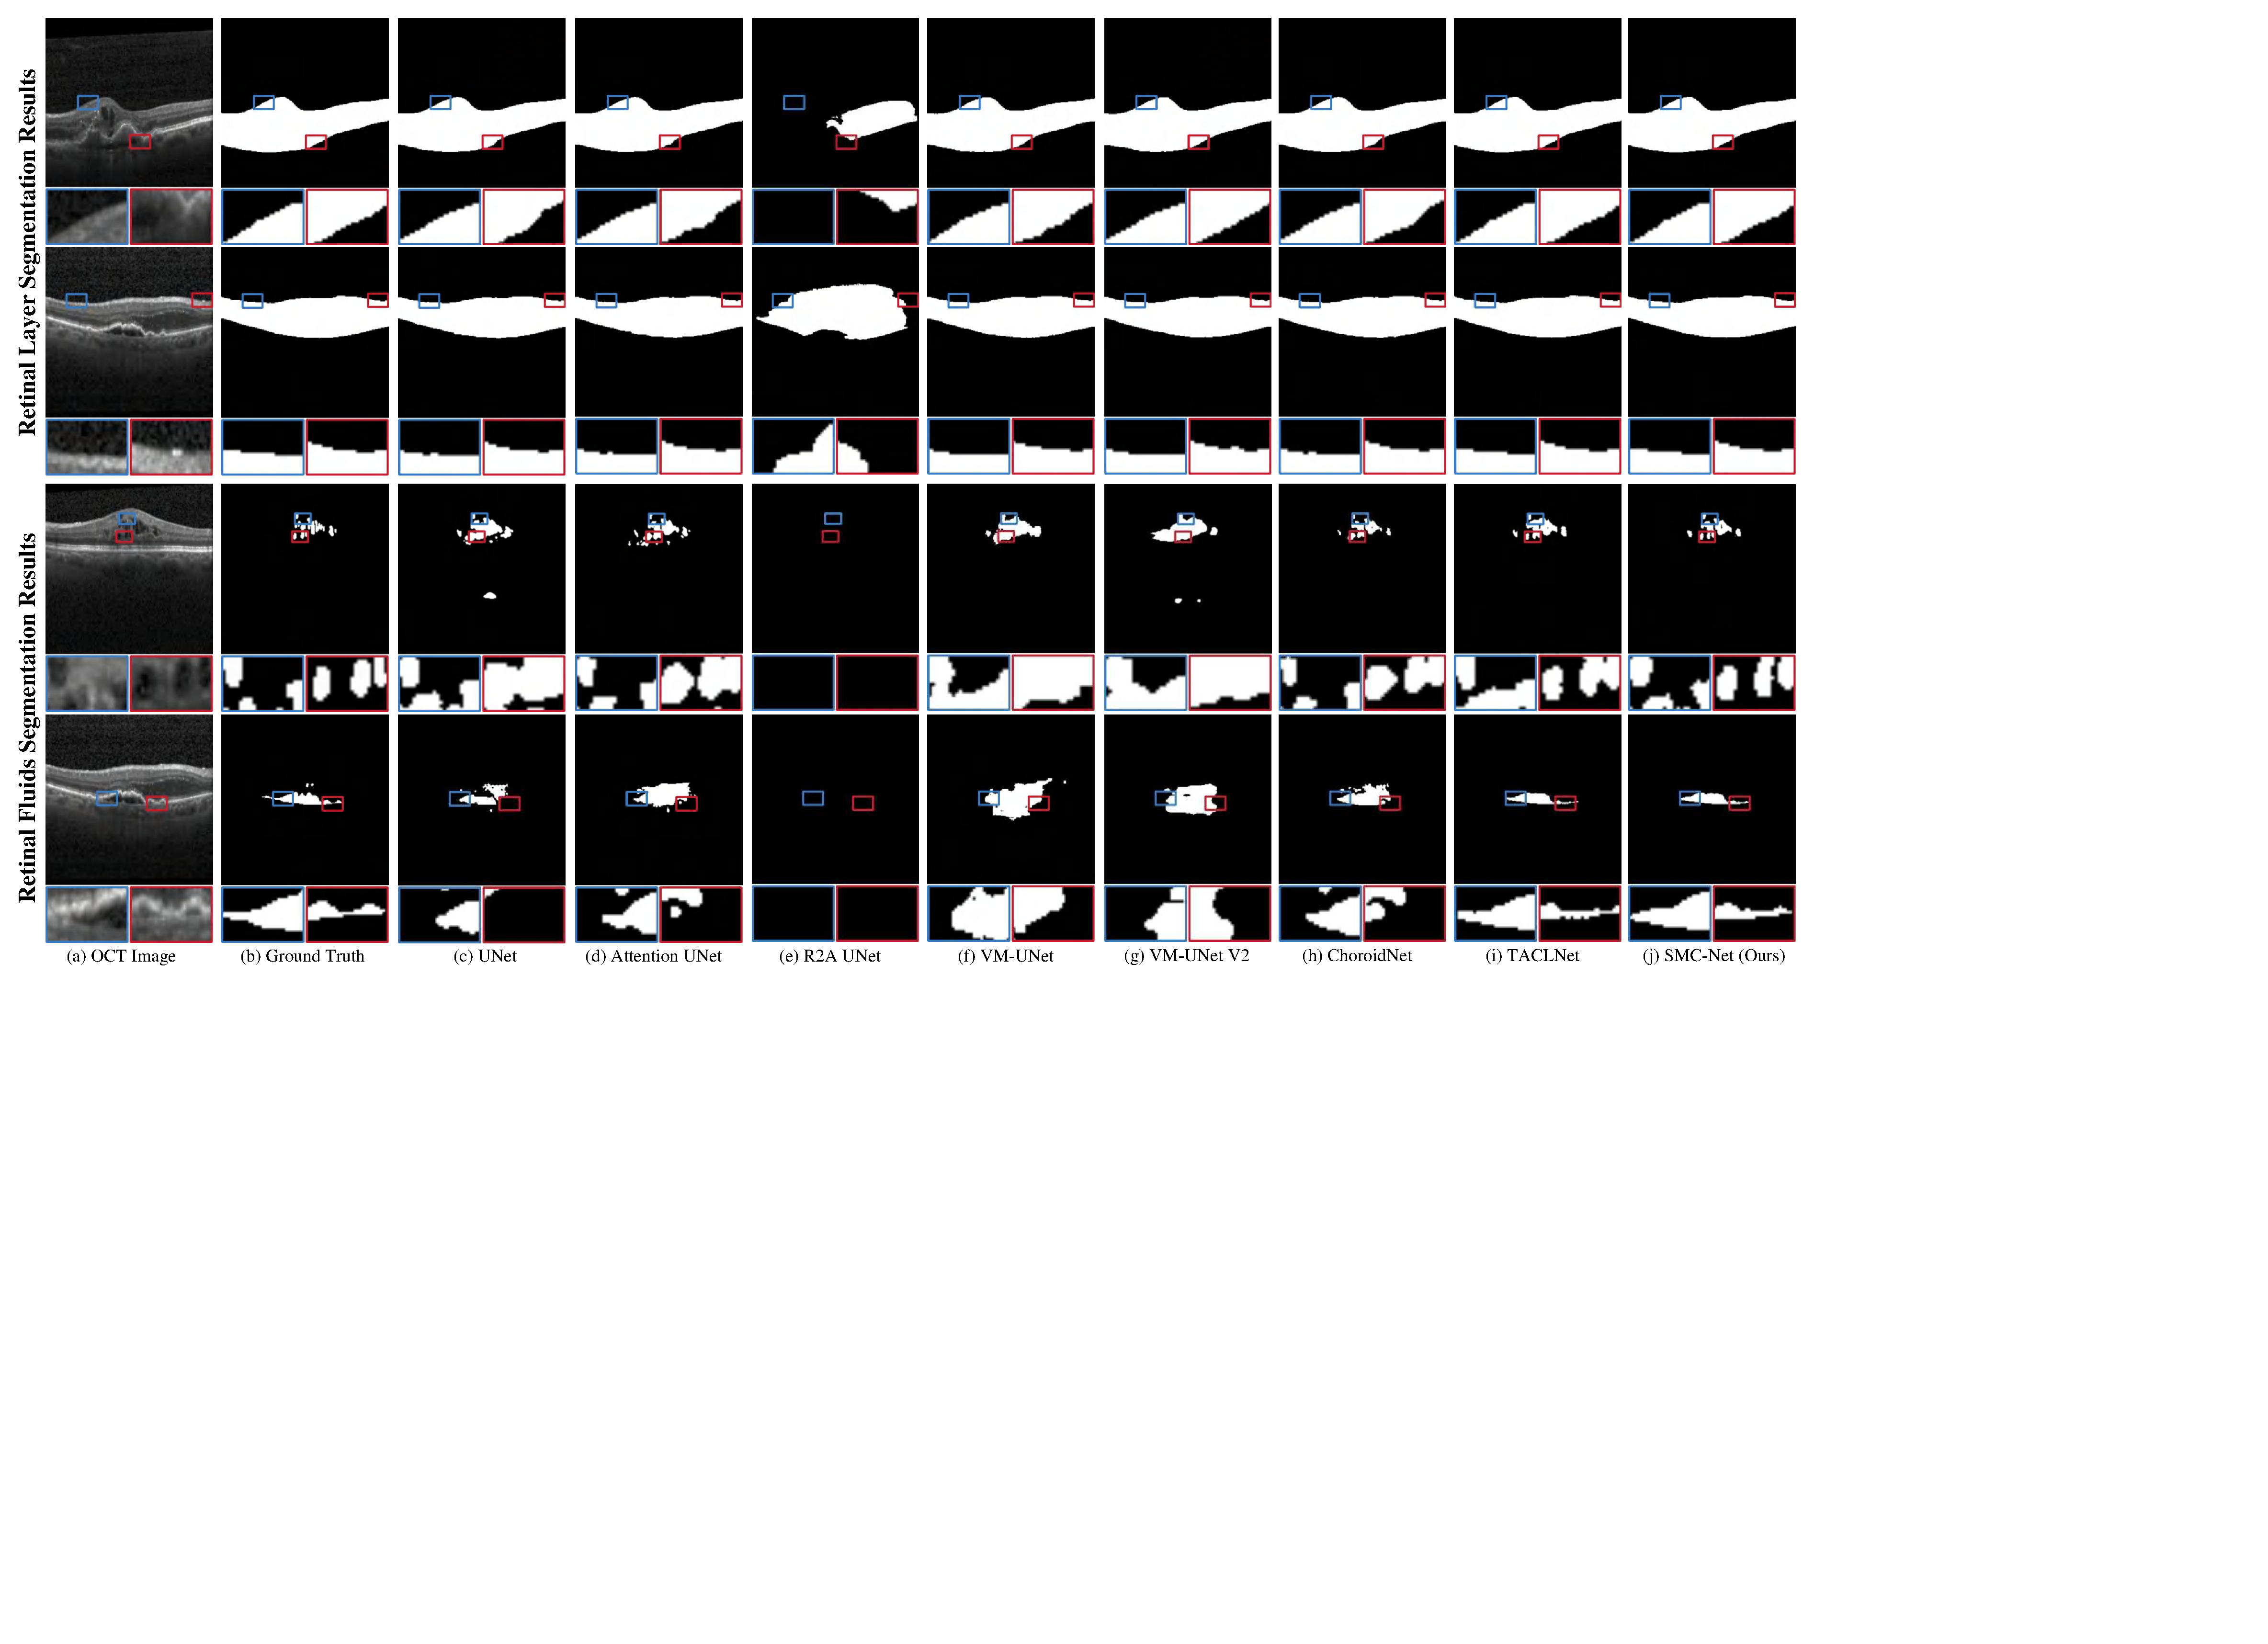
\includegraphics[width=0.9\linewidth]{fig/resultsRetouch.pdf}
    \caption{Qualitative visualization on the public dataset RETOUCH~\cite{RETOUCH}. The top two rows show the segmentation visualizations for the retinal layer, and the bottom two rows show the segmentation visualizations for the retinal fluids. (a) OCT image, (b) Ground Truth, (c) UNet~\cite{ronneberger2015u}, (d) Attention UNet~\cite{Oktay2018AttentionUNet}, (e) R2A UNet~\cite{R2AU-Net}, (f) VM-UNet~\cite{vmunet}, (g) VM-UNet V2~\cite{vmunetv2}, (h) ChoroidNet~\cite{choroidnet}, (i) TACLNet~\cite{wen2024}, (j) SMC-Net (Ours). Below each image, a zoomed-in view of the highlighted area (red and blue boxes) is provided to facilitate the observation of differences.}
    \label{fig:resultsRetouch}
\end{figure*}

\subsection{Implementation Details}
All OCT images were resized to $512\times512$ during both training and inference.
The proposed method was implemented in PyTorch.
To alleviate overfitting, standard data augmentation strategies including random flipping and rotation were applied.
The model was trained for 200 epochs using the AdamW optimizer with a batch size of 4 and an initial learning rate of $1\times10^{-3}$.
The learning rate was scheduled via CosineAnnealingLR with a minimum value of $1\times10^{-5}$.
All experiments were performed on a workstation equipped with an Intel Xeon Silver 4310 CPU and two NVIDIA GeForce RTX 4090 D GPUs.
Segmentation performance was evaluated using the mean Intersection over Union (mIoU), Dice Similarity Coefficient (DSC), Accuracy (Acc), Specificity (Spe), and Sensitivity (Sen), with higher values indicating better performance.

\subsection{Experiment Results}
We evaluate the proposed SMC-Net on our private OCT-CCV dataset and its extended version, and compare it with a wide range of competitive methods.
The compared approaches include:
(i) CNN-based segmentation models, such as U-Net~\cite{ronneberger2015u}, Attention U-Net~\cite{Oktay2018AttentionUNet}, R2U-Net~\cite{alom2018recurrentresidualconvolutionalneural}, R2AU-Net~\cite{R2AU-Net}, and CVI-Net~\cite{cvinet};
(ii) state-space-model-based methods, including H-vmUNet~\cite{wu2024hvmunethighordervisionmamba}, Ultralight VM-UNet~\cite{wu2024ultralightvmunetparallelvision}, VM-UNet~\cite{vmunet}, and VM-UNetV2~\cite{vmunetv2};
and (iii) methods specifically designed for choroidal segmentation, such as ChoroidNet~\cite{choroidnet} and TACLNet~\cite{wen2024}.

\subsubsection{Results on the OCT-CCV Dataset}
\textbf{Quantitative Results}: We conduct 5-fold cross-validation on the OCT-CCV dataset, and report the results in Table~\ref{tab:oct_ccv}.
Overall, the proposed SMC-Net consistently achieves state-of-the-art performance in both choroidal layer and vessel segmentation.
In particular, SMC-Net-S improves the best competing results by 0.04--2.09\% for choroidal layer segmentation and 0.09--0.37\% for vessel segmentation.
Moreover, SSM-based methods (e.g., VM-UNet and VM-UNetV2) generally outperform CNN-based models (e.g., U-Net and Attention U-Net), highlighting the benefit of enhanced long-range dependency modeling.
{\color{red}
Under the same training and evaluation protocol (identical data splits, augmentation strategies, optimizers, training epochs, and input resolution), R2UNet and R2AUNet failed to converge stably on the OCT-CCV dataset in multiple cross-validation runs, resulting in degenerate predictions.
To avoid potential misinterpretation, the corresponding mIoU scores are not reported in Table~\ref{tab:oct_ccv}.
Other CNN baselines trained normally under the same setting, indicating that the instability is likely related to the recurrent residual design when applied to noisy choroidal OCT data.
}

\textbf{Qualitative Analysis}: Fig.~\ref{fig:resultsOctccv} presents representative qualitative comparisons on the OCT-CCV dataset.
While most methods produce reasonable results for choroidal layer segmentation due to its relatively smooth structure, SMC-Net yields more complete and consistent contours, especially in the central convex regions.
For the more challenging vessel segmentation task, SMC-Net demonstrates clear advantages, including improved robustness to noise and artifacts and more accurate delineation of fine vessel boundaries.
In contrast, competing methods often misclassify dark background regions as vessels or fail to recover subtle vascular structures.

\subsubsection{Results on the RETOUCH Dataset}
\textbf{Quantitative Results}: We further evaluate the robustness of SMC-Net on the public RETOUCH dataset~\cite{RETOUCH} using 5-fold cross-validation, with quantitative results summarized in Table~\ref{tab:retouch} and representative examples shown in Fig.~\ref{fig:resultsRetouch}.
Overall, SMC-Net achieves competitive performance in both retinal layer and retinal edema segmentation.
For retinal layer segmentation, all methods exhibit comparable performance, which can be attributed to the relatively clear anatomical boundaries and high-quality annotations in RETOUCH.
In contrast, retinal edema segmentation reveals more pronounced differences: choroid-specialized or cascaded frameworks, such as ChoroidNet~\cite{choroidnet} and TACLNet~\cite{wen2024}, demonstrate better generalization than conventional medical segmentation models, highlighting the importance of anatomical priors for this task.

\textbf{Qualitative Results}:
Qualitative comparisons further support these observations.
As shown in Fig.~\ref{fig:resultsRetouch}, most methods accurately delineate retinal layers due to their smooth contours and high contrast.
However, for the more challenging retinal edema segmentation, non-cascaded models are often affected by interference from irrelevant retinal structures and semantic confusion.
In comparison, our cascaded joint segmentation framework effectively leverages retinal layer predictions as anatomical priors and, through joint optimization, achieves more accurate and consistent edema segmentation.

\section{Ablation Studies}
\subsection{Scaling Trends of Computational Complexity and Performance}


\begin{figure}[!h]
    \centering
    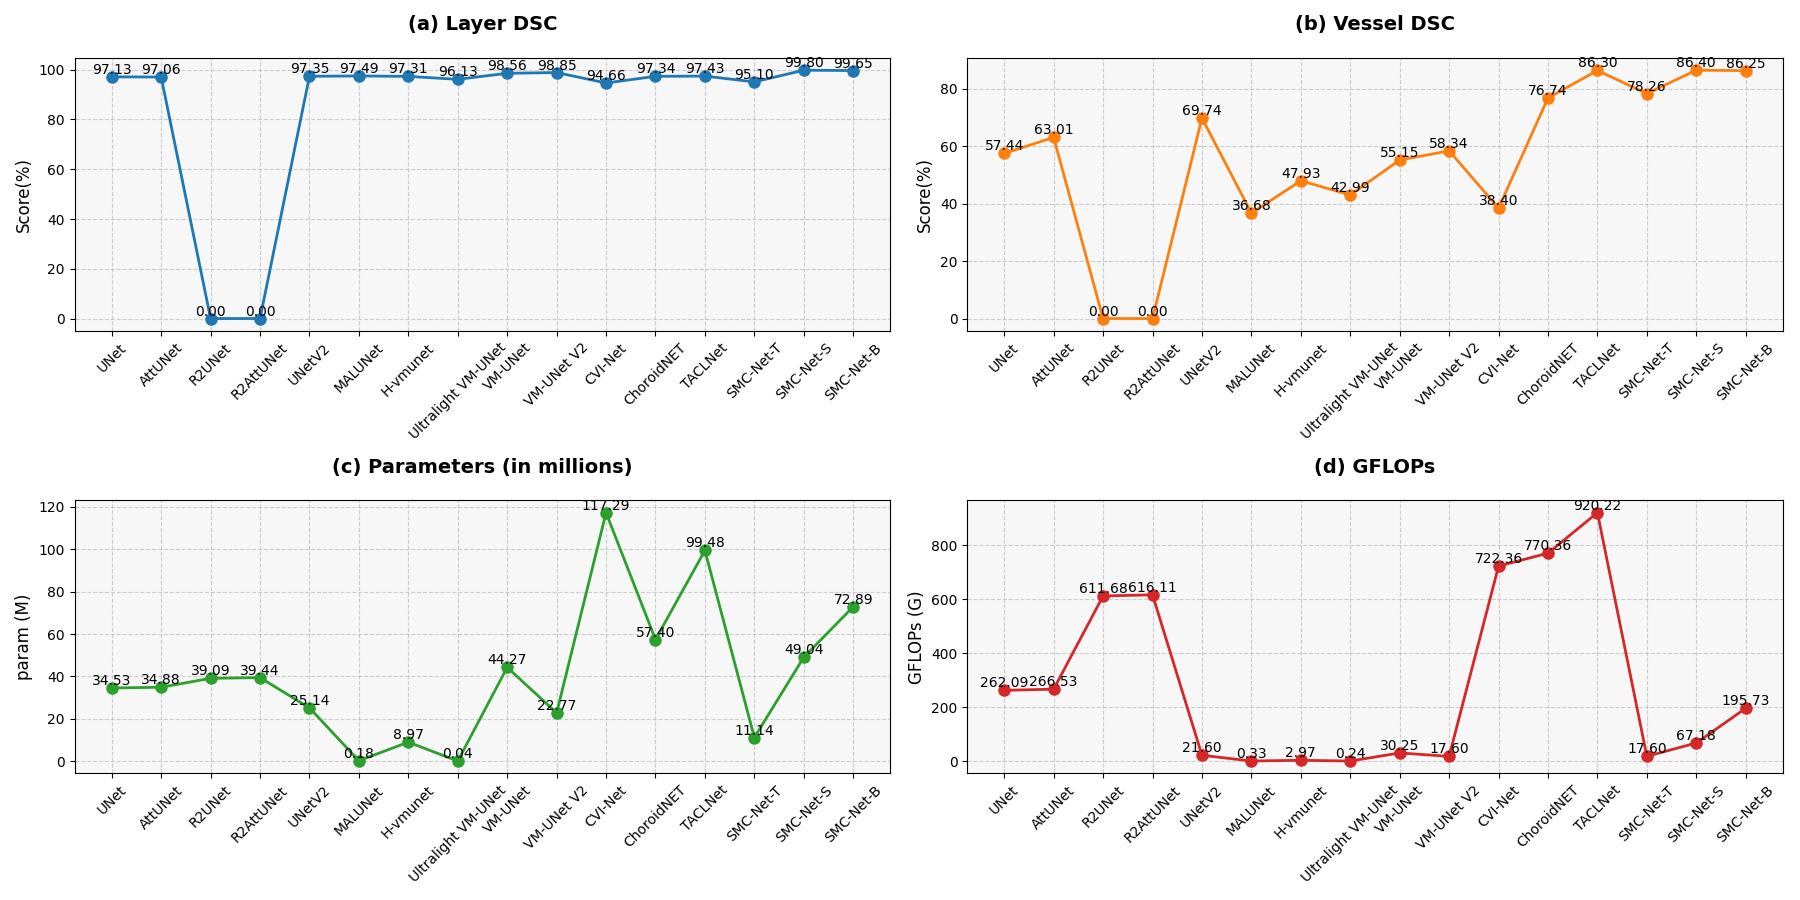
\includegraphics[width=1\linewidth]{fig/complexity_compare.png}
    \caption{Accuracy--efficiency trade-off on OCT-CCV ($512\times512$, batch=1, fp32). (a) Layer DSC, (b) Vessel DSC, (c) Params (M), (d) GFLOPs (G).}
    \label{fig:complexity_compare}
\end{figure}

\textbf{Architecture and FLOPs Scaling}: In addition to segmentation accuracy, we compare model complexity in terms of parameter count and GFLOPs on the OCT-CCV dataset.
As shown in Fig.~\ref{fig:complexity_compare}, the proposed SMC-Net series consistently achieves a favorable accuracy--efficiency trade-off.
In particular, SMC-Net-S attains the best choroidal layer and vessel DSC while maintaining moderate model size and computational cost.
Compared with the Transformer-based TACLNet~\cite{wen2024}, SMC-Net-S achieves comparable or better performance with approximately half the parameters and nearly one order of magnitude fewer GFLOPs.
Moreover, performance gains saturate beyond SMC-Net-S (49.04M parameters), indicating diminishing returns from further model scaling.


\begin{table}[!h]
\renewcommand{\arraystretch}{1.15}
\centering
\begingroup\color{red}\small
\setlength{\tabcolsep}{4pt}
\caption{Inference-time breakdown of the SMC-Net series on OCT-CCV ($512\times512$, fp32, batch=1) with an RTX 4090 D. SMC-Net-S is measured; SMC-Net-T/B are estimated by scaling the measured network time (coarse+refine) linearly with GFLOPs while keeping UPED fixed at $0.8$~ms.}
\label{tab:inference_time_smcnet}  
\resizebox{\linewidth}{!}{
\begin{tabular}{@{}lcccccc@{}}
\toprule
Variant & Params (M) & GFLOPs (G) & UPED (ms) & Coarse+Refine (ms) & Total (ms) & FPS \\ \midrule
SMC-Net-T & 11.14 & 17.60 & 0.8 & 3.1 & 3.9 & 257 \\
SMC-Net-S & 49.04 & 67.18 & 0.8 & 11.8 & 12.6 & 79 \\
SMC-Net-B & 72.89 & 195.73 & 0.8 & 34.4 & 35.2 & 28 \\ \bottomrule
\end{tabular}
}
\endgroup
\end{table}
\textbf{Inference Time}: We further evaluate inference efficiency on a single NVIDIA RTX 4090 D GPU (batch size 1, $512\times512$, fp32).
SMC-Net-S processes one OCT image in 12.6~ms (approximately 79 FPS), demonstrating its suitability for real-time or near-real-time deployment.
Table~\ref{tab:inference_time_smcnet} reports the inference-time breakdown of the SMC-Net series, showing consistent scaling behavior across Tiny, Small, and Base variants.

\begin{figure}[!h]
\centering
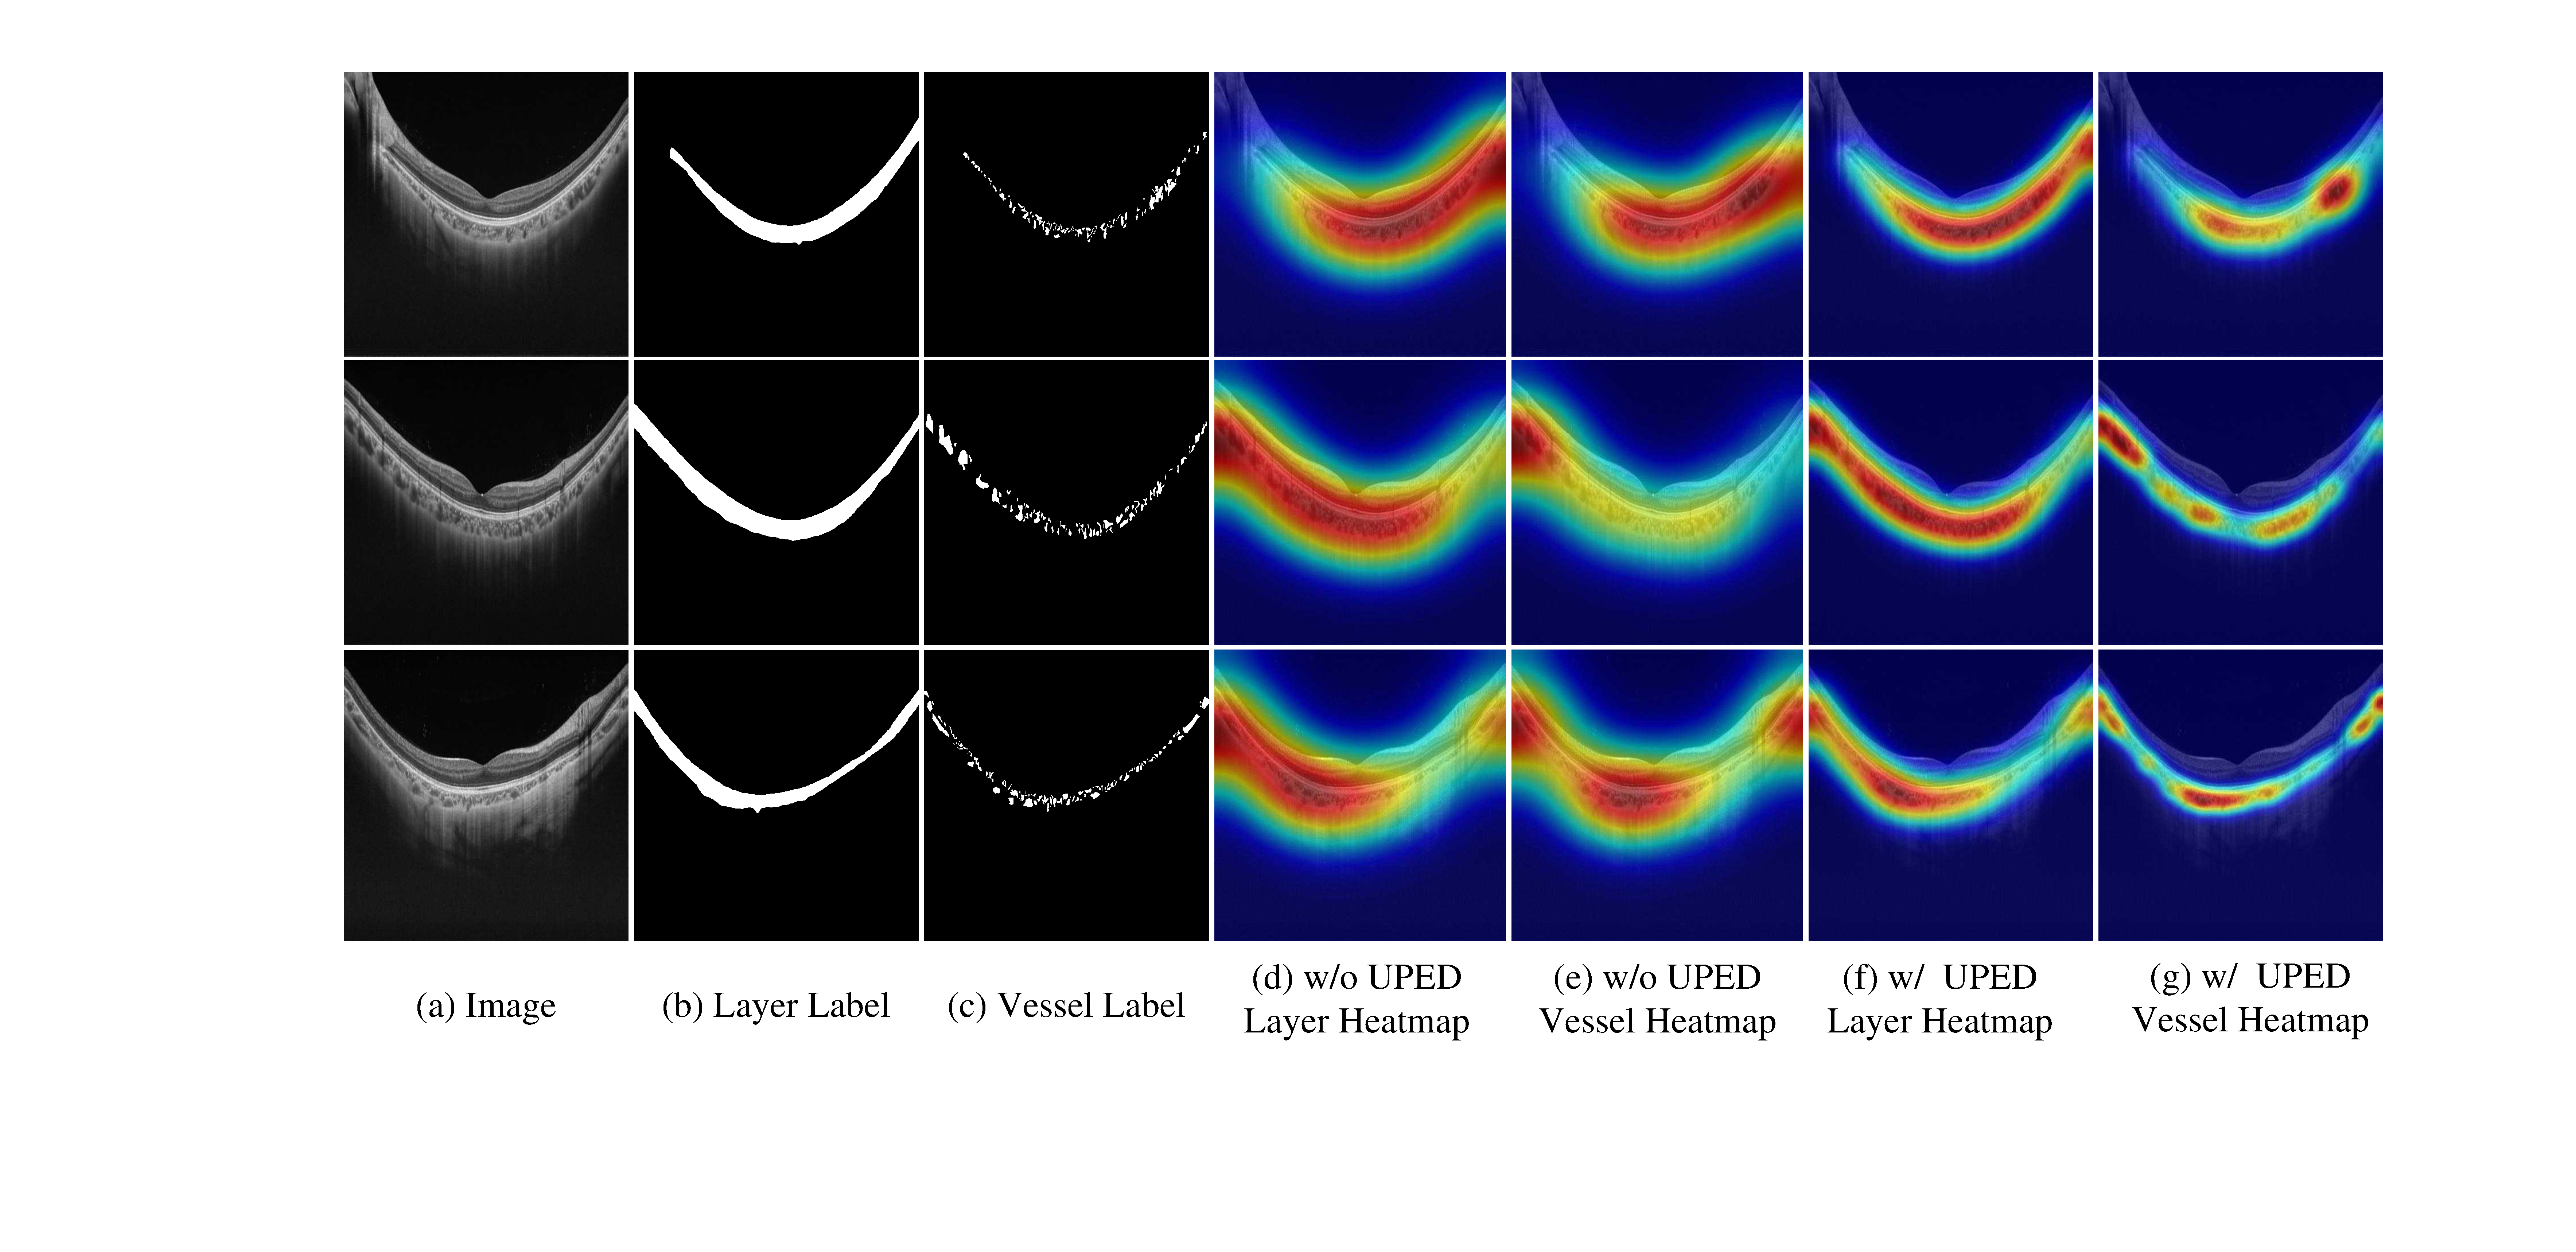
\includegraphics[width=1\linewidth]{fig/ablation_2.pdf}
\caption{Visualization of decoder attention with and without UPED.
(a) Input image, (b) choroidal layer ground truth, (c) vessel ground truth,
(d) attention map of the layer decoder without UPED,
(e) attention map of the vessel decoder without UPED,
(f) attention map of the layer decoder with UPED,
and (g) attention map of the vessel decoder with UPED.
UPED enhances decoder focus on complex vascular regions, leading to more informative and structure-aware representations.}
\label{fig:ablation_decoder_attn}
\end{figure}

\begin{table}[h!]
\centering
\caption{Ablation comparison of different edge detection methods on the OCT-CCV dataset using SMC-Net-S for choroidal vessel segmentation. Best results are shown in \textbf{bold}.}
\label{tab:ablation_detector_compare}
\renewcommand{\arraystretch}{1.15}
\resizebox{\linewidth}{!}{
\begin{tabular}{lccccc}
\hline
\multirow{2}{*}{\textbf{Settings}} & \multicolumn{5}{c}{\textbf{Metrics on OCT-CCV}} \\ \cline{2-6} 
 & \textbf{mIoU(\%)↑} & \textbf{DSC(\%)↑} & \textbf{Acc(\%)↑} & \textbf{Spe(\%)↑} & \textbf{Sen(\%)↑} \\ \hline
Sobel & 72.14 & 83.41 & 99.17 & 99.21 & 82.53 \\
Canny & 71.01 & 82.52 & 99.10 & 99.01 & 81.56 \\ \hline
Multi-dir. Sobel~\cite{dual_encoder_edge} & 73.12 & 83.65 & 99.18 & 99.28 & 82.40 \\ \hline
Zhou \textit{et al.}~\cite{Zhou_2023_CVPR} & 71.34 & 82.81 & 99.06 & 99.08 & 81.73 \\
Ce. \textit{et al.}~\cite{cetinkaya2024ranked} & 71.03 & 82.57 & 99.11 & 99.07 & 81.34 \\ \hline
Ours & \boldmath$75.58$ & \boldmath $86.40$ & \boldmath $99.30$ & \boldmath $99.64$ & \boldmath $84.83$ \\ \hline
\end{tabular}
}
\end{table}

\subsection{Effectiveness of the Unsupervised Prior Edge Detector}
{\color{red}
We evaluate the effectiveness of the proposed Unsupervised Prior Edge Detector (UPED) by replacing the structural modality with the original OCT image during the refinement stage.
As shown in Table~\ref{tab:ablation_1} (Rows 1--2), introducing UPED consistently improves segmentation performance, yielding gains of 2.29\% in mIoU, 1.61\% in DSC, 0.22\% in Acc, 0.17\% in Spe, and 1.40\% in Sen.
The decoder attention visualizations in Fig.~\ref{fig:ablation_decoder_attn} further indicate that UPED guides the network to focus on vascular regions rather than the entire choroid, facilitating more discriminative vessel segmentation.

We further compare UPED with classical and learning-based edge detection methods by injecting different edge modalities into SMC-Net under identical settings.
As reported in Table~\ref{tab:ablation_detector_compare}, traditional Sobel and Canny operators yield limited improvements, while the multi-directional Sobel method~\cite{dual_encoder_edge} achieves better performance (73.12/83.65 mIoU/DSC).
In contrast, UPED attains the best results (75.58/86.40 mIoU/DSC), with comparable Acc, Spe, and Sen.
These results suggest that the fractional-differential formulation of UPED is more effective at preserving weak vascular structures and suppressing noise in OCT images, leading to more informative structural priors for choroidal vessel segmentation.
}

\subsection{Fractional-order Sensitivity}
{\color{red}
We analyze the sensitivity of the fractional-order parameter $v$ in UPED by sweeping $v\in\{0.2,0.4,0.6,0.8\}$ on the OCT-CCV validation folds.
Across this range, vessel DSC varies by less than 0.3\%, with the best performance achieved at $v=0.6$, which is fixed for all experiments without dataset-specific tuning.
Lower values ($v=0.2$--$0.4$) slightly under-emphasize weak vessel edges, while a higher value ($v=0.8$) introduces mild noise amplification. However, none of these settings destabilize training.

UPED employs a fixed set of four canonical orientations ($0^\circ,45^\circ,90^\circ,135^\circ$) and aggregates them into an omni-directional response, eliminating the need for angle tuning.
These results indicate that UPED exhibits low sensitivity to hyperparameter choices and remains robust and reproducible across varying OCT noise levels and imaging conditions.
}

\subsection{Comparison between SSSD and VSSD}
\begin{table}[!h]
\centering
\begingroup\color{red}
\caption{SSSD vs. VSSD comparison on OCT-CCV dataset(SMC-Net-T/S/B, vessel segmentation target).}
\label{tab:sssd_vssd}
\resizebox{\linewidth}{!}{
\begin{tabular}{lllll}
\toprule
Backbone & Params (M) & GFLOPs (G) & mIoU (\%) $\uparrow$ & DSC (\%) $\uparrow$ \\ \midrule
SMC-Net-T w/ VSSD~\cite{shi2024vssdvisionmambanoncausal} & 6.96 & 11.00 & 71.82 & 82.74 \\
SMC-Net-T (SSSD, Ours) & 11.14 & 17.60 & \textbf{73.10} & \textbf{84.12} \\ \midrule
SMC-Net-S w/ VSSD~\cite{shi2024vssdvisionmambanoncausal} & 30.65 & 41.99 & 74.21 & 85.02 \\
SMC-Net-S (SSSD, Ours) & 49.04 & 67.18 & \textbf{75.58} & \textbf{86.40} \\ \midrule
SMC-Net-B w/ VSSD~\cite{shi2024vssdvisionmambanoncausal} & 45.56 & 122.33 & 74.64 & 85.41 \\
SMC-Net-B (SSSD, Ours) & 72.89 & 195.73 & \textbf{76.02} & \textbf{86.78} \\ \bottomrule
\end{tabular}
}
\endgroup
\end{table}
{\color{red}
To evaluate the benefit of the proposed Spatiocanal State Space Duality (SSSD) over the Vision State Space Duality (VSSD) block~\cite{shi2024vssdvisionmambanoncausal}, we replace all SSSD blocks in SMC-Net-T/S/B with VSSD while keeping other components unchanged.
Table~\ref{tab:sssd_vssd} reports the corresponding parameters, GFLOPs, mIoU, and DSC on the OCT-CCV dataset. Across all model scales, SSSD consistently achieves higher segmentation accuracy at the cost of increased model complexity.
For example, on SMC-Net-S, replacing SSSD with VSSD results in performance drops of 1.37\% mIoU and 1.38\% DSC, while reducing parameters and GFLOPs by approximately 1.6$\times$.
These results indicate that jointly modeling spatial and channel-wise dependencies enables SSSD to better capture layer--vessel co-variation in choroidal OCT images than the spatial-only VSSD design, thereby justifying its higher computational cost.
}

\begin{figure}[!h]
    \centering
    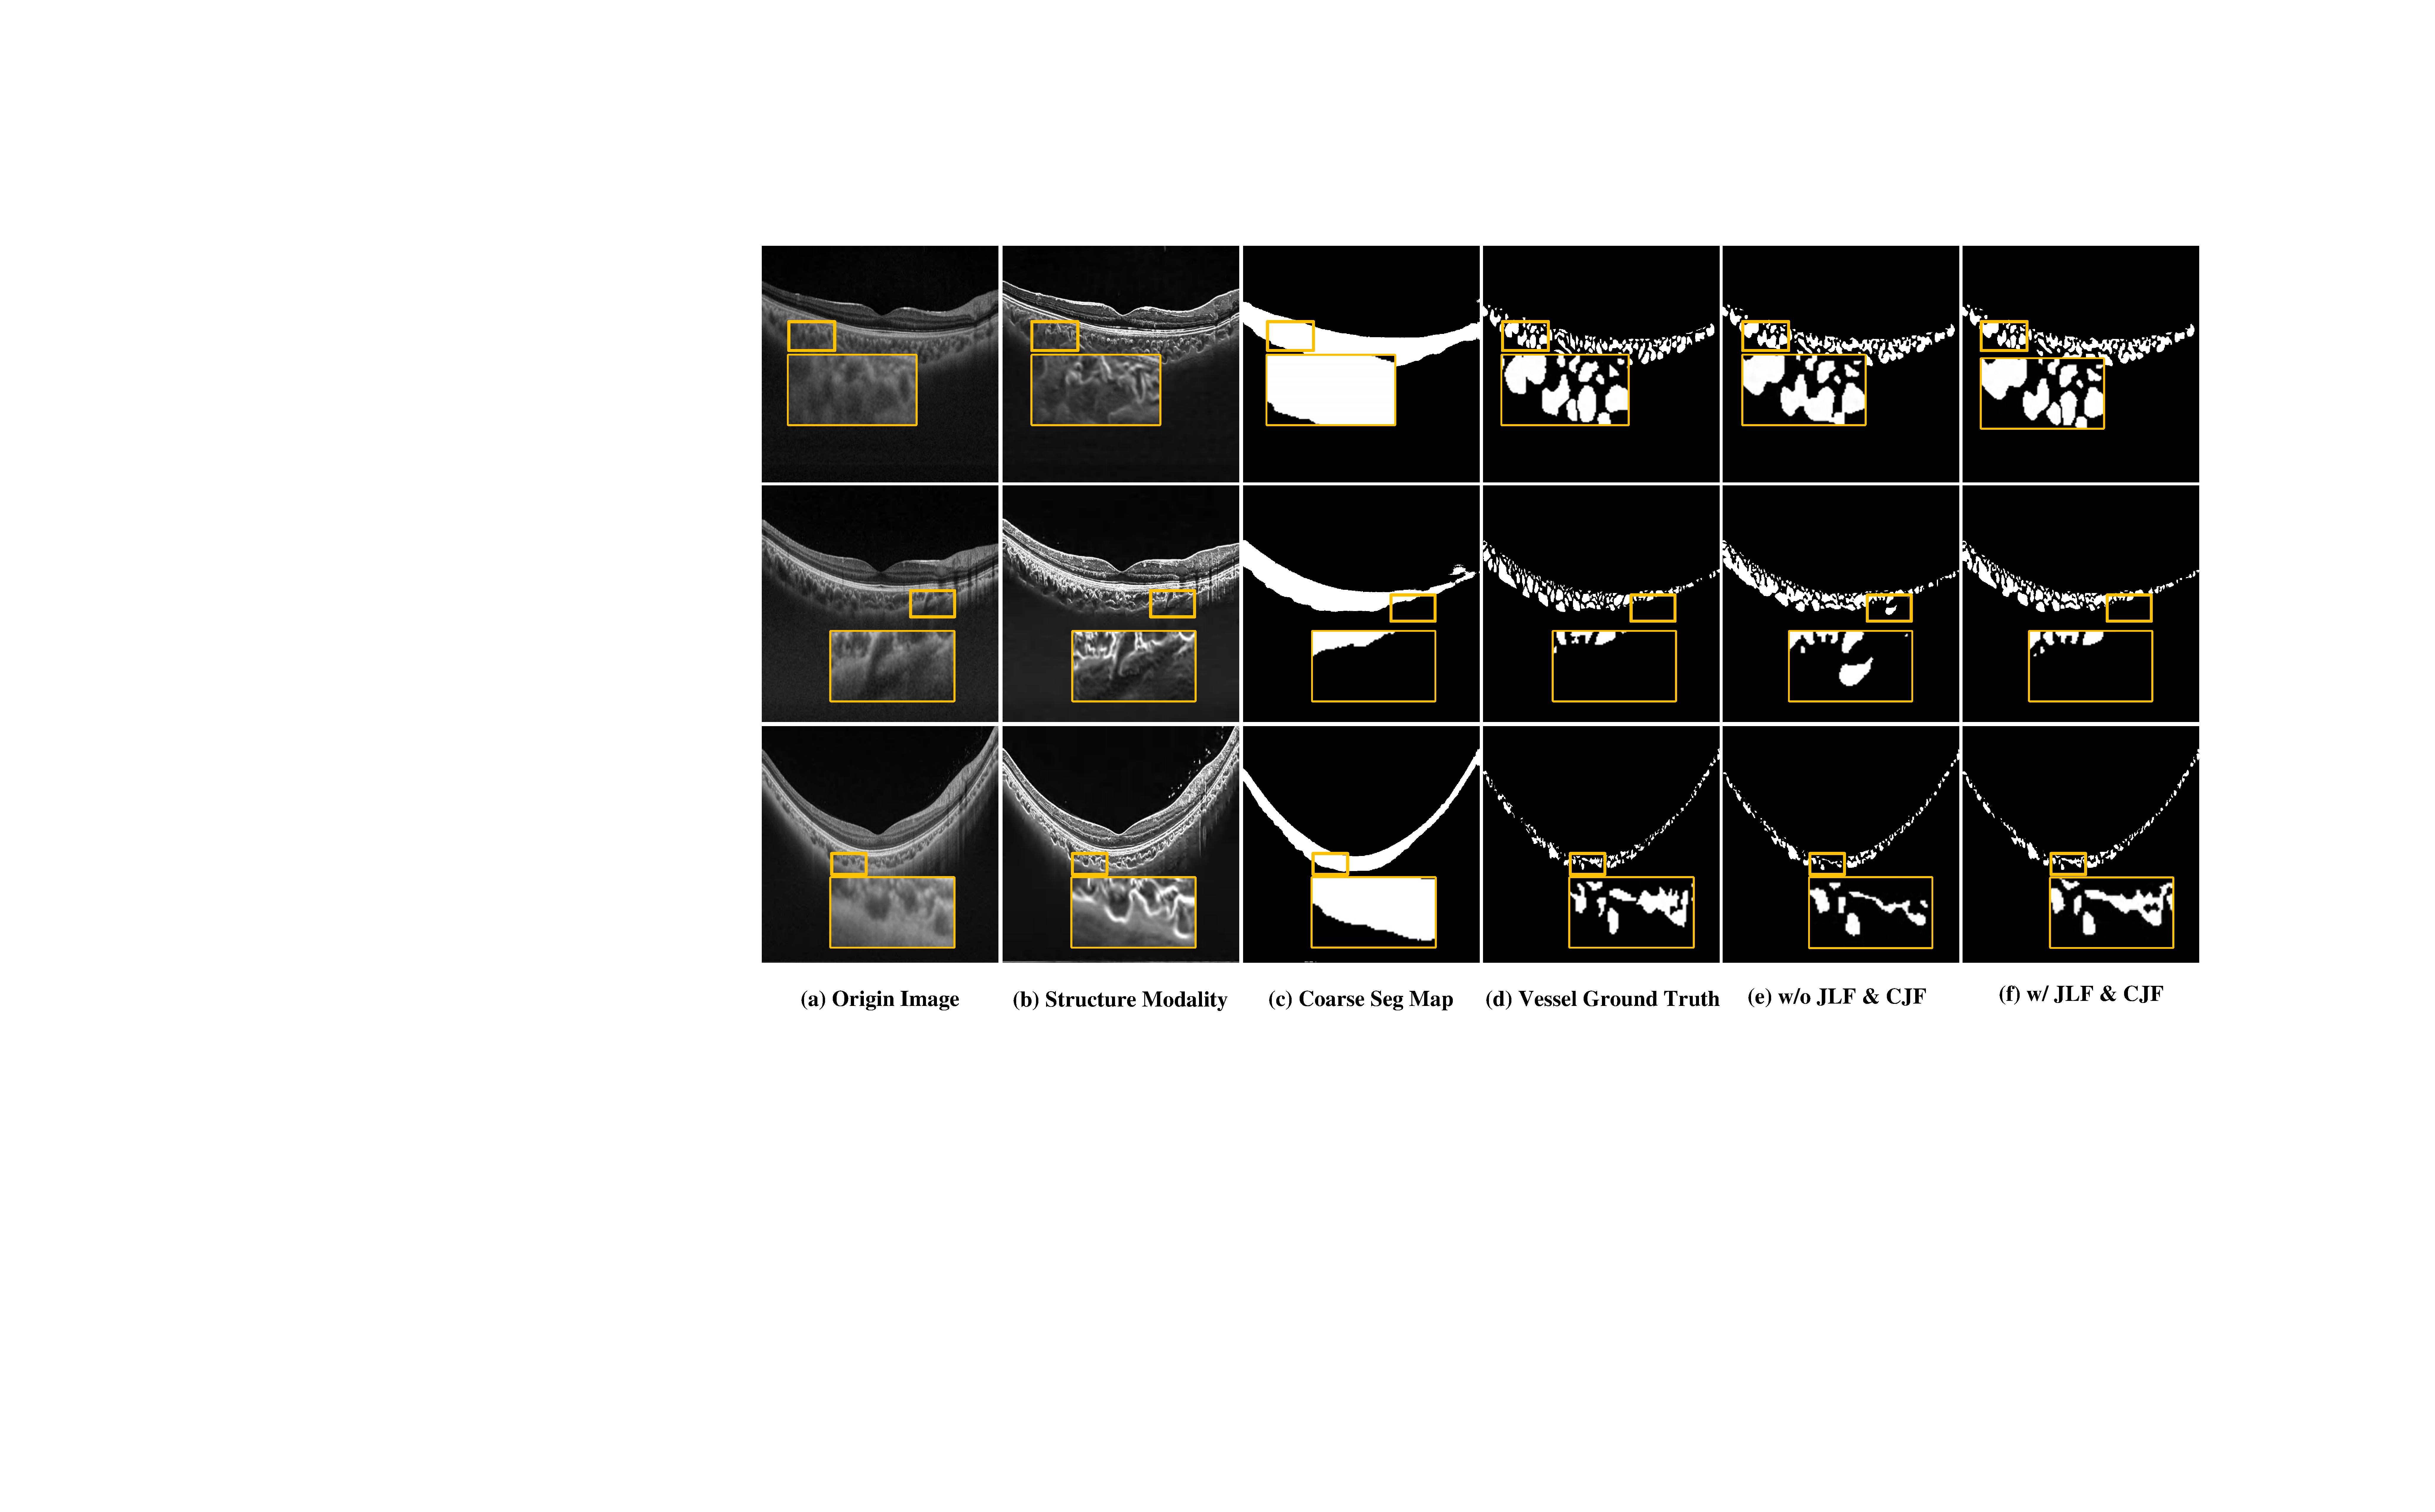
\includegraphics[width=1\linewidth]{fig/ablation_jlf_cjf.pdf}
    \caption{Qualitative comparison illustrating the effect of the Joint Loss Function (JLF) and Cascaded Joint Framework (CJF) in SMC-Net.
    (a) Original OCT image, (b) structural prior extracted by UPED, (c) coarse choroidal segmentation, (d) ground truth, (e) prediction without JLF and CJF, and (f) prediction with JLF and CJF.
    The proposed joint modeling effectively suppresses artifacts and improves vessel boundary consistency.}
    \label{fig:ablation_joint}
\end{figure}

\begin{table}[!h]
\renewcommand{\arraystretch}{1.2}
\centering
\caption{Ablation results ($mean \pm std$) on the OCT-CCV dataset for choroidal vessel segmentation with SMC-Net-S. Best results are shown in \textbf{bold}.}
\label{tab:ablation_1}
\resizebox{\linewidth}{!}{
\begin{tabular}{cccccccc}
\hline
\multicolumn{3}{l}{\textbf{Settings}} & \multirow{2}{*}{\textbf{mIoU(\%)↑}} & \multirow{2}{*}{\textbf{DSC(\%)↑}} & \multirow{2}{*}{\textbf{Acc(\%)↑}} & \multirow{2}{*}{\textbf{Spe(\%)↑}} & \multirow{2}{*}{\textbf{Sen(\%)↑}} \\ \cline{1-3}
w/ UPED & w/ JLF & w/ CJF &  &  &  &  &  \\ \hline
 &  &  & 66.29 & 77.20 & 98.32 & 97.65 & 70.03 \\
$\checkmark$ &  &  & 68.58 & 78.81 & 98.54 & 97.82 & 71.43 \\
$\checkmark$ & $\checkmark$ &  & 70.18 & 80.39 & 98.80 & 98.14 & 72.80 \\
$\checkmark$ & $\checkmark$ & $\checkmark$ & \boldmath $75.58$ & \boldmath $86.40$ & \boldmath $99.30$ & \boldmath $99.64$ & \boldmath $84.83$ \\ \hline
\end{tabular}
}
\end{table}

\subsection{Effectiveness of Joint Anatomical Modeling}
{\color{red}
We conduct ablation studies to examine whether explicitly modeling the anatomical dependency between choroidal layers and vessels improves segmentation performance.
To isolate the effect of the Joint Loss Function (JLF), it is replaced with the Dice--BCE loss, while the Cascaded Joint Framework (CJF) is ablated by removing the pretrained coarse segmentation stage and the choroidal layer decoder in the refinement stage.
Quantitative results in Table~\ref{tab:ablation_1} (Rows 3--4) demonstrate consistent performance improvements.
Specifically, JLF improves mIoU, DSC, Acc, Spe, and Sen by 1.60\%, 1.59\%, 0.26\%, 0.32\%, and 1.40\%, respectively, while CJF yields larger gains of 5.40\%, 7.00\%, 0.50\%, 1.50\%, and 12.03\%.
Qualitative comparisons in Fig.~\ref{fig:ablation_joint} further show that CJF and JLF effectively suppress imaging artifacts and enhance vessel segmentation fidelity.

We further analyze the contribution of UPED relative to the architectural components.
Adding UPED alone to a plain backbone improves vessel DSC from 77.20\% to 78.81\% (+1.61\%), whereas the full SMC-Net configuration (UPED + SSSD + MCAM + SAM + JLF/CJF) achieves 86.40\% DSC.
Edge ablation results also indicate that UPED outperforms a multi-directional Sobel operator by 2.75\% DSC.
These results suggest that while UPED provides effective structural priors, the majority of performance gains arise from the proposed joint anatomical modeling, which integrates long-range feature modeling, structure-aware fusion, and boundary-level constraints to fully exploit such priors.
}
\section{Discussion}
{\color{red}
Clinically, accurate joint segmentation of choroidal layers and vessels in swept-source OCT enables quantitative analysis of choroidal thickness and vascular indices, which are relevant to diseases such as myopia and age-related macular degeneration. By producing layer-aware vessel maps that are robust to noise and artifacts, SMC-Net may support longitudinal analysis and treatment response evaluation, and can serve as a preprocessing module for downstream clinical applications. Despite these advantages, the current method is limited to 2D B-scans and may degrade under extremely poor image quality or unseen acquisition conditions. Future work will explore volumetric modeling and improved robustness across devices and datasets.
}
\section{Conclusion}
{\color{red}
In this paper, we propose \textbf{SMC-Net}, a structure-aware cascaded framework for choroidal vessel segmentation in OCT images.
By integrating Spatiocanal State Space Duality for efficient long-range modeling with a fractional-differential-based unsupervised edge prior for structural enhancement, SMC-Net enables anatomically consistent joint segmentation of choroidal layers and vessels.
Extensive experiments on both private and public datasets demonstrate that SMC-Net consistently outperforms existing methods in terms of accuracy and efficiency, supporting its potential utility for quantitative choroidal analysis in both clinical and research settings.
}

\bibliographystyle{ieeetr} 
\bibliography{reference}

\end{document}
